% =====================================================================
%  Final Dissertation Report - Dimpal Shetty (2024MT13052)
%  Follows "Guidelines for preparation of WILP Project Report (06.04.2022)"
%    - 9" x 11" page, 1" margins, double spacing, one side, serial page numbers
%    - small Roman page numbers before the Introduction, Arabic from it onwards
%    - decimal section numbering (1, 1.1, 1.1.1)
%  Compile with pdfLaTeX (Overleaf default). Run twice so the table of
%  contents, lists and glossary page numbers fill in.
%
%  Anything shown in RED on a yellow box is a placeholder you must fill in.
%  Search this file for  \fillin  to find all of them.
% =====================================================================
\documentclass[12pt,oneside]{report}

\usepackage[paperwidth=9in,paperheight=11in,margin=1in,headheight=15pt,includefoot]{geometry} % includefoot: page number stays inside the 1" margin
\usepackage[T1]{fontenc}
\usepackage[utf8]{inputenc}
\usepackage{lmodern}
\usepackage{setspace}          % double spacing (floats stay single spaced)
\usepackage{graphicx}
\usepackage{booktabs}
\usepackage{tabularx}
\usepackage{longtable}
\usepackage{array}
\usepackage{xcolor}
\usepackage{amsmath}
\usepackage{caption}
\usepackage{enumitem}
\usepackage{titlesec}
\usepackage[hidelinks]{hyperref}

\graphicspath{{figures/}}
\captionsetup{font=small,labelfont=bf}
\setlist{nosep,leftmargin=*}
\newcolumntype{L}{>{\raggedright\arraybackslash}X}
\setlength{\emergencystretch}{3em}
\setlength{\parindent}{0pt}         % no first-line indent anywhere (consistent look)
\setlength{\parskip}{6pt}           % small gap between paragraphs instead   % lets long words/numbers wrap instead of sticking out

% Chapter headings: "1. Introduction" instead of the large "Chapter 1" block
\titleformat{\chapter}[hang]{\Large\bfseries}{\thechapter.}{0.6em}{}
\titlespacing*{\chapter}{0pt}{0pt}{18pt}

% ---- Currency. "Rs." always compiles. To show the rupee sign instead,
% ---- add \usepackage{tfrupee} and change the line below to \rupee\,
\newcommand{\INR}{Rs.\,}

% ---- Placeholder marker: anything you still need to fill in
\newcommand{\fillin}[1]{\colorbox{yellow}{\textcolor{red}{\textbf{[#1]}}}}

% ---- Glossary helper: marks where a term is first explained, so the
% ---- glossary at the end can show the page number (as the guidelines ask)
\newcommand{\gl}[2]{\phantomsection\label{gl:#1}#2}

% ---- Details used on the cover, title page and abstract sheet
\newcommand{\ReportTitle}{DEMAND FORECASTING IN INVENTORY MANAGEMENT}
\newcommand{\StudentName}{Dimpal Shetty}
\newcommand{\StudentID}{2024MT13052}
\newcommand{\Discipline}{M.Tech. Software Systems}
\newcommand{\CourseNo}{S1-26\_SSZG628T}
\newcommand{\OrgName}{Airbus India Pvt Ltd}
\newcommand{\OrgPlace}{Bengaluru}
\newcommand{\SubmitMonth}{November 2026}

\begin{document}

% =====================================================================
%  COVER  (Appendix A of the guidelines) - no page number
% =====================================================================
\pagenumbering{gobble}
\begin{titlepage}
\centering\singlespacing
\vspace*{1.2in}
{\large\bfseries A REPORT\par}\vspace{0.6em}
{\large\bfseries ON\par}\vspace{0.6em}
{\Large\bfseries \ReportTitle\par}
\vspace{1.4in}
{\large\bfseries BY\par}\vspace{1.2em}
\begin{tabular*}{\textwidth}{@{\extracolsep{\fill}}ll}
\textbf{\StudentName} & \textbf{ID No.: \StudentID}
\end{tabular*}
\vspace{1.2in}

{\large\bfseries AT\par}\vspace{1em}
{\bfseries Bengaluru, Karnataka\par}\vspace{0.4em}
{\bfseries \OrgName, \OrgPlace\par}
\vfill
{\bfseries BIRLA INSTITUTE OF TECHNOLOGY \& SCIENCE, PILANI\par}\vspace{0.4em}
{\bfseries \SubmitMonth\par}
\end{titlepage}

% =====================================================================
%  TITLE PAGE  (Appendix B) - first numbered page, small Roman numerals
% =====================================================================
\pagenumbering{roman}
\setcounter{page}{1}
\begin{titlepage}
\thispagestyle{plain}
\centering\singlespacing
\vspace*{0.8in}
{\large\bfseries A REPORT\par}\vspace{0.6em}
{\large\bfseries ON\par}\vspace{0.6em}
{\Large\bfseries \ReportTitle\par}
\vspace{1.2in}
{\large\bfseries BY\par}\vspace{1.2em}
\begin{tabular*}{\textwidth}{@{\extracolsep{\fill}}lll}
\textbf{\StudentName} & \textbf{ID No.: \StudentID} & \textbf{\Discipline}
\end{tabular*}
\vspace{0.9in}

Prepared in partial fulfilment of the\\
WILP Dissertation Course (\CourseNo)
\vspace{0.9in}

{\large\bfseries AT\par}\vspace{1em}
{\bfseries \OrgName, \OrgPlace\par}
\vfill
{\bfseries BIRLA INSTITUTE OF TECHNOLOGY \& SCIENCE, PILANI\par}\vspace{0.4em}
{\bfseries \SubmitMonth\par}
\end{titlepage}
\setcounter{page}{2}

% =====================================================================
%  ACKNOWLEDGEMENTS  (order as given in the guidelines)
% =====================================================================
\doublespacing
\chapter*{Acknowledgements}
\addcontentsline{toc}{chapter}{Acknowledgements}

I am grateful to my supervisor, Saurabh Mahajan, HO of Architecture, \OrgName, for the direction, time and honest feedback given at every stage of the project.

I thank my additional examiner, Karthik Mahadevan, Digital Sourcing Lead, \OrgName, for reviewing my work and for the helpful suggestions.

I thank my faculty mentor, Ashish Narang, BITS Pilani, for the guidance and support given throughout this dissertation.

I also thank my manager, PhaniKiran Vemagal, \OrgName, for supporting me in carrying out this work alongside my role.

\vspace{2em}
\noindent\StudentName\\
\StudentID

% =====================================================================
%  ABSTRACT SHEET  (Appendix C) - abstract kept under 200 words
% =====================================================================
\clearpage
\phantomsection
\addcontentsline{toc}{chapter}{Abstract Sheet}
\begin{singlespace}
\begin{center}
{\bfseries BIRLA INSTITUTE OF TECHNOLOGY AND SCIENCE, PILANI\\(RAJASTHAN)\\WILP Division\par}
\end{center}
\vspace{0.5em}
\noindent
\begin{tabularx}{\textwidth}{@{}>{\raggedright\arraybackslash}p{4.6cm} L@{}}
\textbf{Organization:} & \OrgName \hfill \textbf{Location:} \OrgPlace\\[3pt]
\textbf{Duration:} & 13 weeks \hfill \textbf{Date of Start:} 08 August 2026\\[3pt]
\textbf{Date of Submission:} & 10 November 2026\\[3pt]
\textbf{Title of the Project:} & Demand Forecasting in Inventory Management\\[3pt]
\textbf{ID No./Name of the student:} & \StudentID{} / \StudentName\\[3pt]
\textbf{Name(s) and Designation(s) of Supervisor and Additional Examiner:} &
  Saurabh Mahajan, HO of Architecture, \OrgName{}\newline
  Karthik Mahadevan, Digital Sourcing Lead, \OrgName{}\\[3pt]
\textbf{Name of the Faculty mentor:} & Ashish Narang\\[3pt]
\textbf{Key Words:} & Spare-parts demand forecasting; LightGBM; ABC/XYZ classification; safety stock; Aircraft On Ground (AOG); landing gear; Apriori\\[3pt]
\textbf{Project Areas:} & Predictive Analytics; Machine Learning; Inventory Management\\
\end{tabularx}

\vspace{0.6em}
\noindent\textbf{Abstract:}
Airlines need the right spare parts ready before an aircraft comes in for repair. A missing part can ground the aircraft (Aircraft On Ground, AOG), while too much stock ties up money. Most parts are reordered on fixed schedules. This project builds a data-driven pipeline that forecasts demand for one landing-gear spare part and turns the forecast into a stock decision. It uses a public Kaggle dataset of 10,000 simulated landing records. A value and volatility (ABC/XYZ) classification picked the Landing Gear Actuator as the part worth forecasting. In this data, landing load, not runway condition, drives its failure. A tuned LightGBM model, tested only on batches it had never seen, cut the forecast error from 6.18 to 0.30 units per batch of 200 landings; Random Forest reached 0.10. A cost-based reorder rule then cut the safety buffer from about 23 units to 2, lowering the estimated yearly cost from \INR 2.46 crore to \INR 0.21 crore with no stockouts in the test. Apriori mining found parts that fail together, and a supplier dashboard shows the results. Because the data is simulated, the main contribution is the method; real airline data is needed to confirm the numbers.

\vspace{2.2em}
\noindent
\begin{tabular*}{\textwidth}{@{\extracolsep{\fill}}ll}
\rule{2.2in}{0.4pt} & \rule{2.2in}{0.4pt}\\
Signature of Student & Signature of Supervisor\\
Date: 09-11-2026 & Date: 09-11-2026\\
\end{tabular*}
\end{singlespace}

% =====================================================================
%  CONTENTS, FIGURES, TABLES
% =====================================================================
\clearpage
\begin{singlespace}
\tableofcontents
\clearpage
\phantomsection\addcontentsline{toc}{chapter}{List of Figures}
\listoffigures
\clearpage
\phantomsection\addcontentsline{toc}{chapter}{List of Tables}
\listoftables
\end{singlespace}

% =====================================================================
%  MAIN TEXT - Arabic page numbers start here
% =====================================================================
\clearpage
\pagenumbering{arabic}
\setcounter{page}{1}

% ---------------------------------------------------------------------
\chapter{Introduction}
\label{ch:intro}
% ---------------------------------------------------------------------

\section{Background}
Airline maintenance teams, known as \gl{mro}{MRO (Maintenance, Repair and Overhaul)} teams, need the right spare parts on the shelf before an aircraft comes in for repair. If a part is missing, the aircraft cannot fly until the part arrives. This is called an \gl{aog}{AOG (Aircraft On Ground)} event. Public industry figures put the cost of an AOG event at roughly US\$10,000 to US\$150,000 per hour, depending on the aircraft and the route.

The opposite mistake is also costly. Keeping many spare parts ``just in case'' ties up money in stock that sits on a shelf. For an expensive part, such as a landing-gear actuator, every extra unit held for a year costs a lot in capital, storage and insurance.

Today, most spare parts are reordered on a fixed schedule based on flight hours or flight cycles. A fixed schedule treats every aircraft the same. It does not look at how each aircraft was actually used, for example how hard it landed or how heavily it was loaded.

\section{Problem statement}
This project addresses the following problem: how can landing-by-landing operating data be used to forecast demand for a high-value landing-gear spare part, and to turn that forecast into a stock decision that balances the cost of running out against the cost of holding stock?

\section{Objectives}
\begin{enumerate}
\item Sort the landing-gear spare parts into priority groups by how much money they account for and how steady their demand is, to decide which part is worth a machine-learning forecast.
\item Build, tune and fairly test a model that forecasts how many units of the chosen part will be needed, using landing conditions as inputs, and compare it against a simple baseline and a second model.
\item Find which spare parts tend to be needed together, so a supplier can bundle them.
\item Turn the forecast into a stock and reorder recommendation in Indian Rupees, weighing the cost of an AOG event against the cost of holding stock.
\item Show the result in a simple dashboard a supplier can use.
\end{enumerate}

\section{Scope}
The project forecasts demand for one part in detail: the Landing Gear Actuator, chosen by the classification in Chapter~\ref{ch:eda}. It uses one public dataset of 10,000 landing records (Chapter~\ref{ch:data}). Live flight data, weather feeds and real Airbus production data are outside the scope. Two companion parts named in the original project outline, seal kits and structural bolts, are not in the dataset and so are not covered.

\section{Methodology in brief}
The work was carried out in seven phases:
\begin{enumerate}
\item Gap analysis and system design.
\item Loading and exploring the data.
\item Baseline forecast, value/volatility classification and companion-part mining.
\item Midterm report.
\item Training and tuning the forecasting models (LightGBM and Random Forest).
\item Building the reorder engine and checking it against the cost model.
\item Building the supplier dashboard and writing this report.
\end{enumerate}
All analysis was done in Python. Every number in this report was produced by the project's Python scripts and can be reproduced by running them.

% ---------------------------------------------------------------------
\chapter{Literature Review and Gap Analysis}
\label{ch:lit}
% ---------------------------------------------------------------------

\section{Spare-parts classification}
Spare-parts classification and demand forecasting is a well-studied area. Bacchetti and Saccani~\cite{bacchetti2012} reviewed the field and found a gap between research and practice: many published methods are tested on idealised data and are rarely checked against real maintenance records. Lagoda and Klumpp~\cite{lagoda2024} proposed a modified ABC-XYZ analysis that links the classification step to the forecasting step instead of treating them separately. This project follows the same idea: the classification result is used to choose which part to forecast. Nafiurridha and Choiruddin~\cite{nafiurridha2024} used supervised machine learning to classify aircraft spare parts. This project keeps the classification simple and easy to explain (ABC/XYZ), and uses machine learning only for the forecast.

\section{Forecasting with usage data}
Olmo and Domingo~\cite{olmo2026} proposed a framework for forecasting demand for aerospace rotable parts. Their main argument is that fleet usage data captures differences in how aircraft are operated, which fixed schedules miss. LightGBM was their best model for most parts. Stanton et al.~\cite{stanton2025} compared hand-chosen machine-learning models with automated machine learning (AutoML) on landing-gear data. This supports comparing more than one model on a landing-gear part, rather than picking one without a test.

\section{Methods used in this project}
The Apriori algorithm of Agrawal and Srikant~\cite{agrawal1994} is the standard method for finding items that occur together, and is used here for companion parts. LightGBM~\cite{ke2017} is a fast gradient-boosting library that builds decision trees one after another, each correcting the errors of the previous ones. Grinsztajn et al.~\cite{grinsztajn2022} showed that tree-based models usually beat deep learning on small and medium tabular datasets like the one used here. Random Forest~\cite{breiman2001}, which averages many independent decision trees, is used as the comparison model. For stock decisions, this project uses the newsvendor rule for safety stock and the economic order quantity (EOQ) for order size, both standard methods in inventory management~\cite{silver2017,harris1913}.

\section{Current practice and the gap}
In current practice:
\begin{itemize}
\item demand is forecast from a fixed flight-hour or flight-cycle schedule, regardless of how each aircraft was used;
\item parts are ranked by yearly cost only, not by how steady their demand is;
\item safety stock is a fixed buffer that is rarely updated;
\item parts are bundled in orders based on engineers' experience, not on measured patterns.
\end{itemize}

Olmo and Domingo~\cite{olmo2026} is the closest study to this one. Compared with that study, this project:
\begin{enumerate}
\item adds a prioritisation step, so that only the part worth forecasting is forecast;
\item measures which operating condition drives failure, with a check that the result does not depend on runway condition;
\item adds companion-part mining for bundled orders;
\item goes all the way to a cost-based stock and order decision and a supplier dashboard.
\end{enumerate}
A clear weakness compared with that study is the data: this project uses a small public simulated dataset, while that study used real fleet data.

% ---------------------------------------------------------------------
\chapter{Dataset and Data Checks}
\label{ch:data}
% ---------------------------------------------------------------------

\section{Source}
The dataset is a public landing-gear maintenance dataset from Kaggle~\cite{kaggle}. The downloaded file is named \texttt{landing\_gear\_maintenance\_simulated\_data.xlsx}. It has 10,000 rows and 12 columns, with no missing values. Each row is one landing. There is no date and no aircraft ID, so landings cannot be linked into the history of one aircraft.

\section{Columns}
Table~\ref{tab:columns} lists the columns. Eight describe the conditions of the landing. Four are yes/no flags that show whether a component showed a failure or wear sign on that landing.

\begin{table}[htbp]
\centering\small
\caption[Dataset columns]{Dataset columns}
\label{tab:columns}
\begin{tabularx}{\textwidth}{@{}lL@{}}
\toprule
\textbf{Column} & \textbf{Meaning}\\
\midrule
\texttt{landing\_cycles} & Number of landing cycles the aircraft had built up\\
\texttt{load\_during\_landing} & Load on the landing gear at touchdown\\
\texttt{taxiing\_duration} & How long the aircraft taxied\\
\texttt{speed\_during\_landing} & Speed at touchdown\\
\texttt{braking\_force} & How hard the brakes were applied\\
\texttt{tire\_pressure} & Tyre pressure at landing\\
\texttt{hydraulic\_pressure} & Hydraulic system pressure\\
\texttt{runway\_condition} & Dry, wet or snowy\\
\midrule
\texttt{brake\_degradation} & 1 if the brake showed wear, else 0\\
\texttt{shock\_absorber\_failure} & 1 if the shock absorber failed, else 0\\
\texttt{tire\_wear} & 1 if the tyre showed wear, else 0\\
\texttt{hydraulic\_system\_failure} & 1 if the hydraulic system failed, else 0\\
\bottomrule
\end{tabularx}
\end{table}

\section{Mapping flags to spare parts}
Each flag was mapped to one spare part (Table~\ref{tab:parts}). This mapping is the author's own choice; it is not given in the data. The rates do not add up to 100\% because each landing has four separate yes/no checks, so one landing can flag several parts. For example, 5,689 landings flag both the actuator and the wheel unit.

\begin{table}[htbp]
\centering\small
\caption[Failure flags mapped to spare parts]{Failure flags mapped to spare parts}
\label{tab:parts}
\begin{tabular}{@{}llr@{}}
\toprule
\textbf{Flag in data} & \textbf{Spare part (author's mapping)} & \textbf{Flag rate}\\
\midrule
\texttt{brake\_degradation} & Brake Assembly & 95.3\%\\
\texttt{shock\_absorber\_failure} & Landing Gear Actuator & 59.7\%\\
\texttt{tire\_wear} & Wheel Unit & 81.7\%\\
\texttt{hydraulic\_system\_failure} & Hydraulic Line & 24.5\%\\
\bottomrule
\end{tabular}
\end{table}

\section{Batches as planning periods}
Because the data has no dates, the 10,000 landings were split, in file order, into 50 \gl{batch}{batches} of 200 landings each. Each batch stands in for one planning period. Under the assumed fleet use of 2,000 landings per year, one batch is about one-tenth of a year (about 36 days). The number of actuator flags in a batch is the ``demand'' for that period. The same batches are used everywhere in this report.

\section{Data check: the failure flags follow fixed rules}
\label{sec:rules}
During model training (Chapter~\ref{ch:model}) the models became almost perfect. This is unusual for real maintenance data, so the data was checked. A small decision tree with only two splits was fitted to each flag. For every flag, a simple two-part rule matched all 10,000 rows exactly (Table~\ref{tab:rules}). Each rule was then checked directly against the data.

\begin{table}[htbp]
\centering\small
\caption[Rules behind each failure flag]{Exact rules behind each failure flag (each matches 10,000 of 10,000 rows)}
\label{tab:rules}
\begin{tabular}{@{}ll@{}}
\toprule
\textbf{Part} & \textbf{Flag = 1 when}\\
\midrule
Landing Gear Actuator & load during landing $>$ 70 \textbf{or} landing cycles $>$ 401\\
Wheel Unit & braking force $>$ 40 \textbf{or} landing cycles $>$ 300\\
Brake Assembly & braking force $>$ 35 \textbf{or} landing cycles $>$ 351.5\\
Hydraulic Line & hydraulic pressure $<$ 2800 \textbf{or} landing cycles $>$ 450.5\\
\bottomrule
\end{tabular}
\end{table}

This shows that the dataset is \gl{sim}{simulated}: the flags were produced by rules, not observed on real aircraft. This has three effects, which are kept in mind throughout the report:
\begin{enumerate}
\item Runway condition is not part of any rule. So the finding that ``landing load matters and weather does not'' (Chapter~\ref{ch:eda}) describes how the simulator was built. It is not proof about real aircraft.
\item The forecasting models can learn these rules exactly, so their errors are close to zero. Real data would contain randomness and the errors would be larger.
\item The value of this project is the \emph{method}: the full pipeline from data to stock decision. Real airline data is needed to confirm the size of the benefit.
\end{enumerate}
The dataset was kept, after discussion, because the pipeline itself does not depend on the data source and can be re-run on real data without changes.

% ---------------------------------------------------------------------
\chapter{System Design and Model Choice}
\label{ch:design}
% ---------------------------------------------------------------------

\section{Architecture}
Figure~\ref{fig:arch} shows how data flows through the system. The main path is always used: the data is prepared, the classification picks the part to forecast, the forecast model predicts demand, and the cost and reorder engine turns the forecast into a stock recommendation shown on the supplier dashboard. Companion-part mining is an optional side branch, shown when a supplier wants bundling suggestions.

\begin{figure}[htbp]
\centering
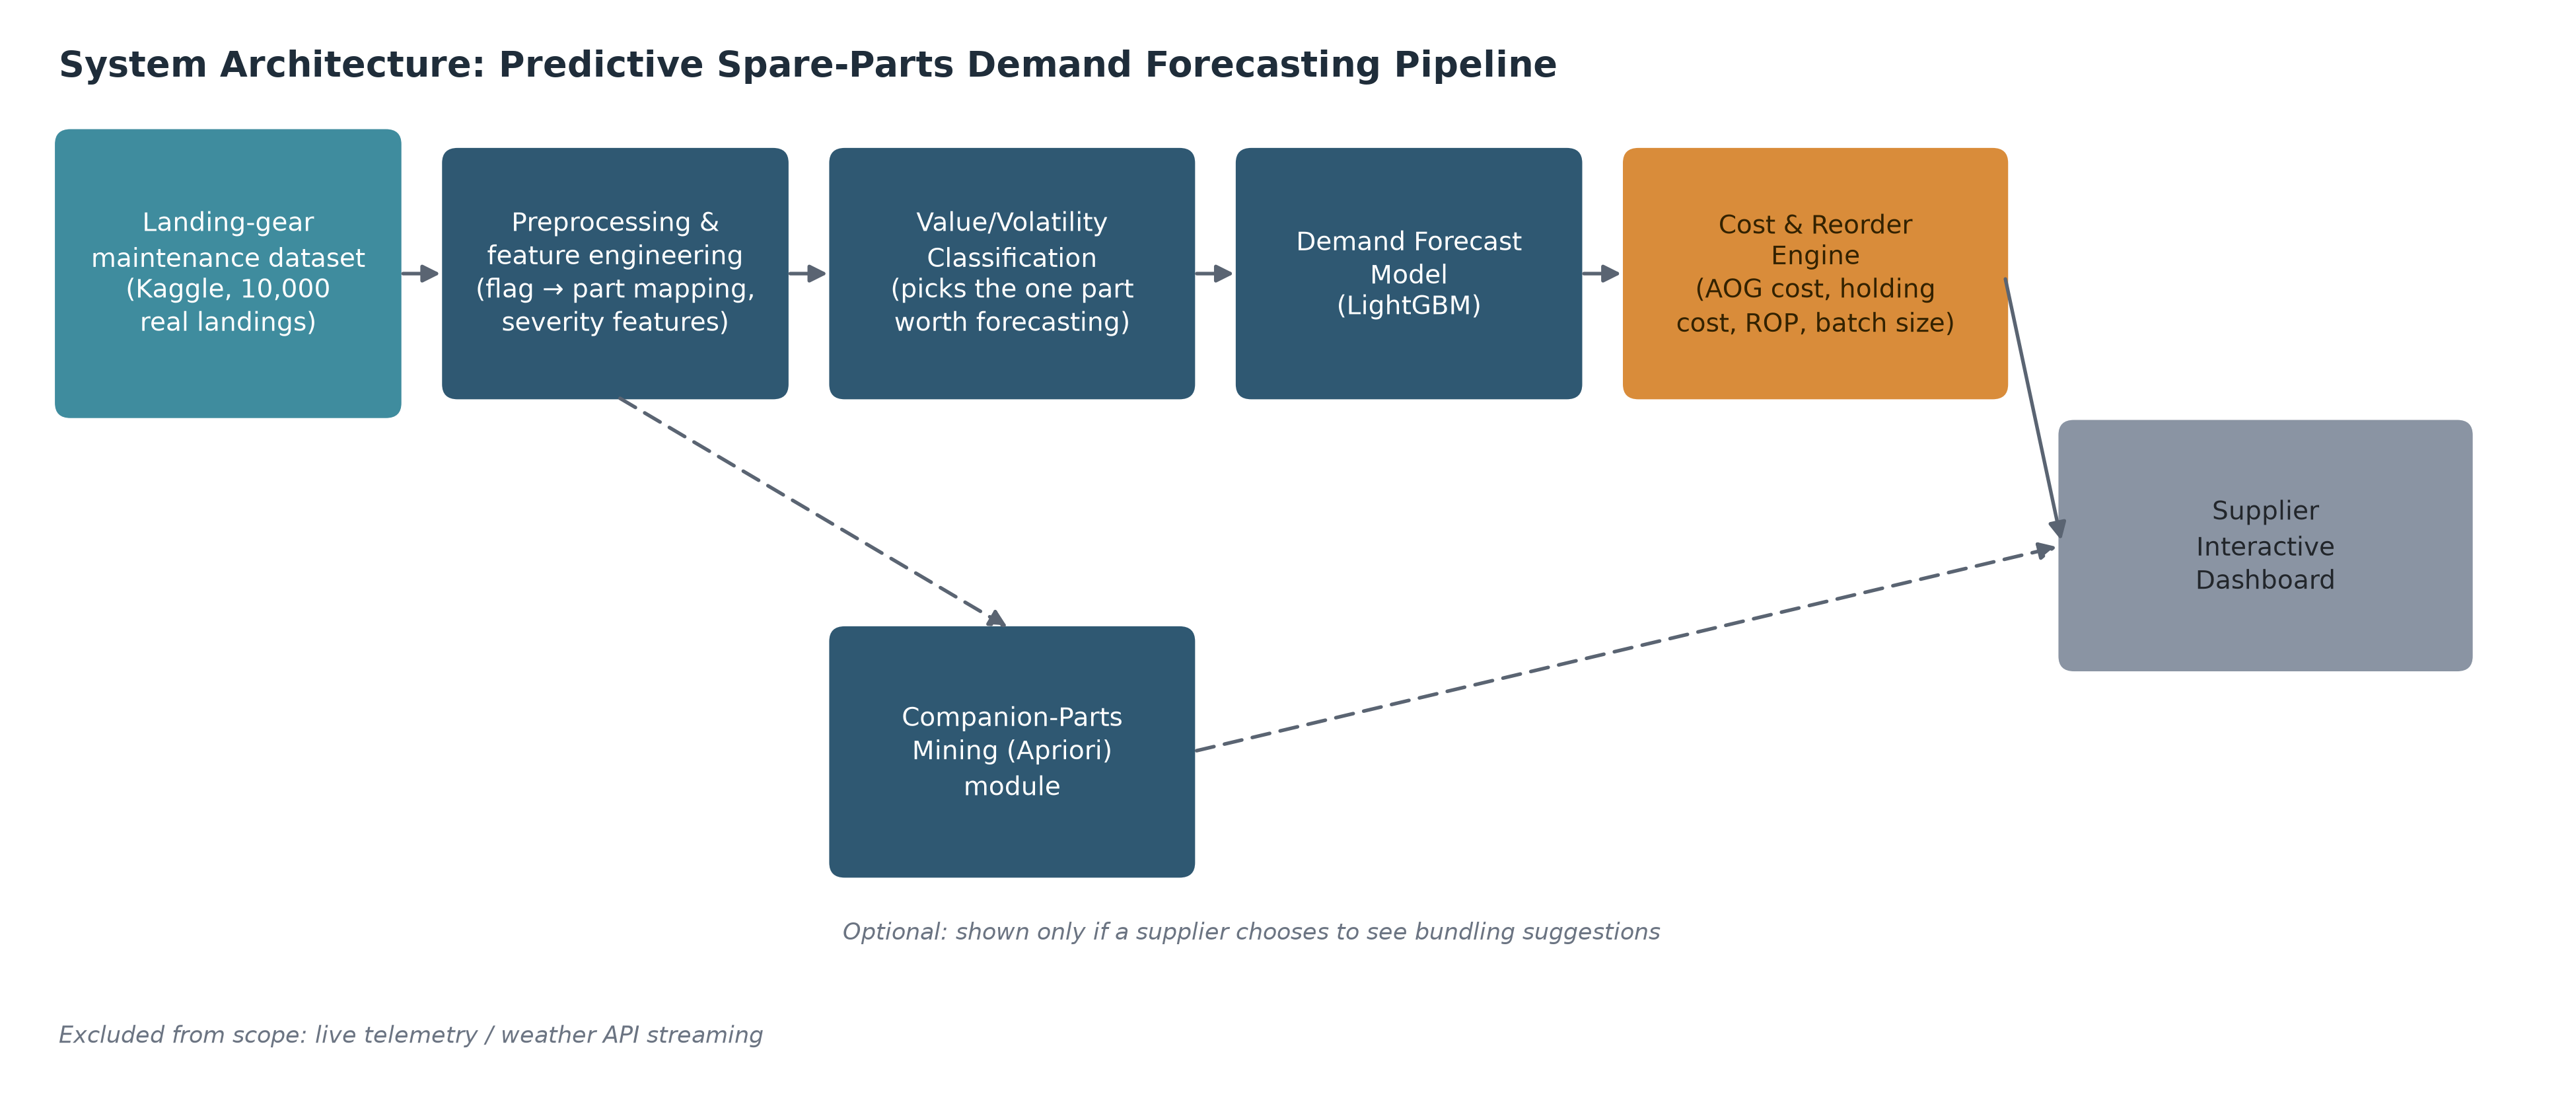
\includegraphics[width=\textwidth]{00_architecture.png}
\caption[System architecture]{System architecture. The solid path is always used; the dashed branch (companion parts) is optional.}
\label{fig:arch}
\end{figure}

\section{Choice of forecasting model}
Table~\ref{tab:models} compares the model families considered.

\begin{table}[htbp]
\centering\small
\caption[Model families considered]{Model families considered}
\label{tab:models}
\begin{tabularx}{\textwidth}{@{}>{\raggedright\arraybackslash}p{3.1cm}LL@{}}
\toprule
\textbf{Model family} & \textbf{How it works} & \textbf{Decision}\\
\midrule
Time-series models (ARIMA, Prophet) & Learn trend and season from a demand series over time. & Not used. The data has no dates, so there is no time series to learn from.\\
Deep learning (LSTM, Transformer) & Neural networks that learn from ordered sequences. & Not used. There is no aircraft ID or date to form sequences, and tree models usually win on small tabular data~\cite{grinsztajn2022}.\\
Random Forest & Averages many decision trees built independently. & Used as the comparison model.\\
LightGBM (gradient boosting) & Builds trees one after another, each fixing the errors of the last. & Chosen as the main model: handles the runway category directly, trains fast, and gives feature importance~\cite{ke2017}. It was the best model in the closest study~\cite{olmo2026}.\\
\bottomrule
\end{tabularx}
\end{table}

LightGBM was chosen as the main model before any training was done, based on the reasons above. Random Forest was trained and tested in exactly the same way so that the choice could be checked.

\section{How the forecast is built}
There are only 50 batches, which is too few rows to train a model directly on batch totals. Instead, the model is trained on all 10,000 individual landings. For each landing, it predicts the \emph{chance} that the actuator flag is 1, using only the eight landing conditions. The other three failure flags are \emph{not} used as inputs, because on a real day they would not be known in advance. The chances for the 200 landings in a batch are then added up. This sum is the forecast number of actuators needed in that batch.

\section{Tools}
The project uses Python 3.12 with pandas for data handling, scikit-learn~\cite{pedregosa2011} for Random Forest and testing, LightGBM 4.6.0, mlxtend~\cite{raschka2018} for Apriori, and matplotlib for charts. The dashboard is a single HTML file with no outside libraries, so it works offline.

% ---------------------------------------------------------------------
\chapter{Data Analysis, Baseline and Prioritisation}
\label{ch:eda}
% ---------------------------------------------------------------------

\section{What drives actuator failure in this data}
Figure~\ref{fig:drivers} compares the actuator flag rate by runway condition and by landing load. Runway condition barely changes the rate: 59.6\% on dry runways, 60.9\% on wet and 58.6\% on snowy. Landing load changes it a lot: the rate rises from near 0\% for the lightest landings to near 100\% for the heaviest.

\begin{figure}[htbp]
\centering
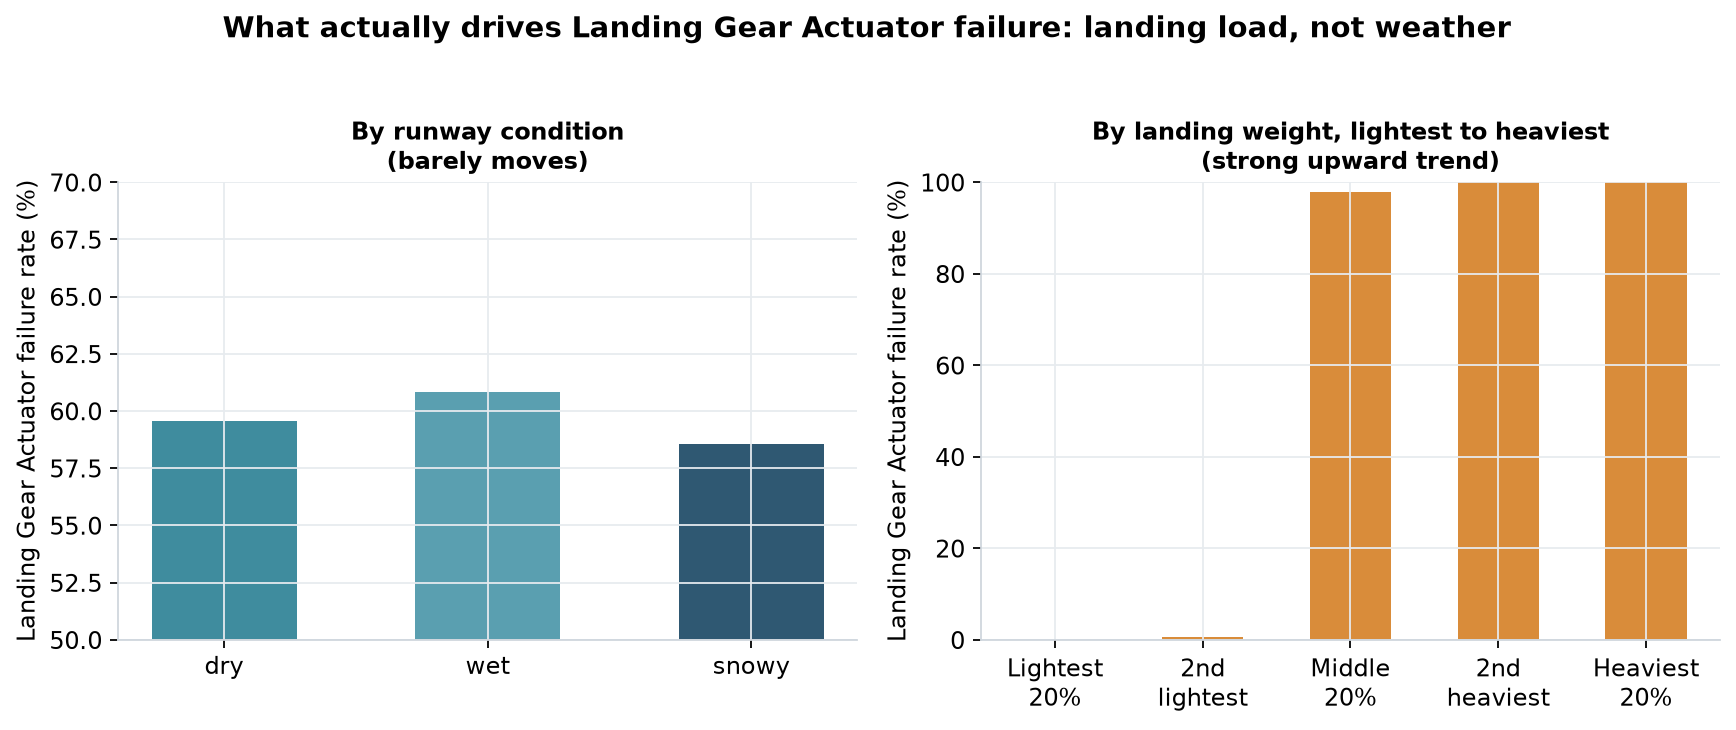
\includegraphics[width=\textwidth]{01_env_brake_temp.png}
\caption[Actuator failure rate by runway condition and landing load]{Actuator flag rate by runway condition (left) and by landing load, lightest to heaviest (right).}
\label{fig:drivers}
\end{figure}

\textbf{Robustness check.} Load might only look important because heavy landings happen more on wet or snowy runways. To test this, the link between load and actuator failure (correlation) was measured separately for each runway condition. It was 0.814 on dry, 0.823 on wet and 0.827 on snowy runways. Since the link is the same in all three groups, runway condition is not hiding behind the load effect.

As explained in Section~\ref{sec:rules}, this result reflects how the simulator was built: runway condition is not in any of its rules. The check is still correct, but it confirms the simulator, not real aircraft behaviour.

\section{Which conditions relate to which part}
Figure~\ref{fig:heat} and Table~\ref{tab:corr} show the correlation between each landing condition and each part's flag. A value near 1 or $-$1 means a strong link; a value near 0 means no link.

\begin{figure}[htbp]
\centering
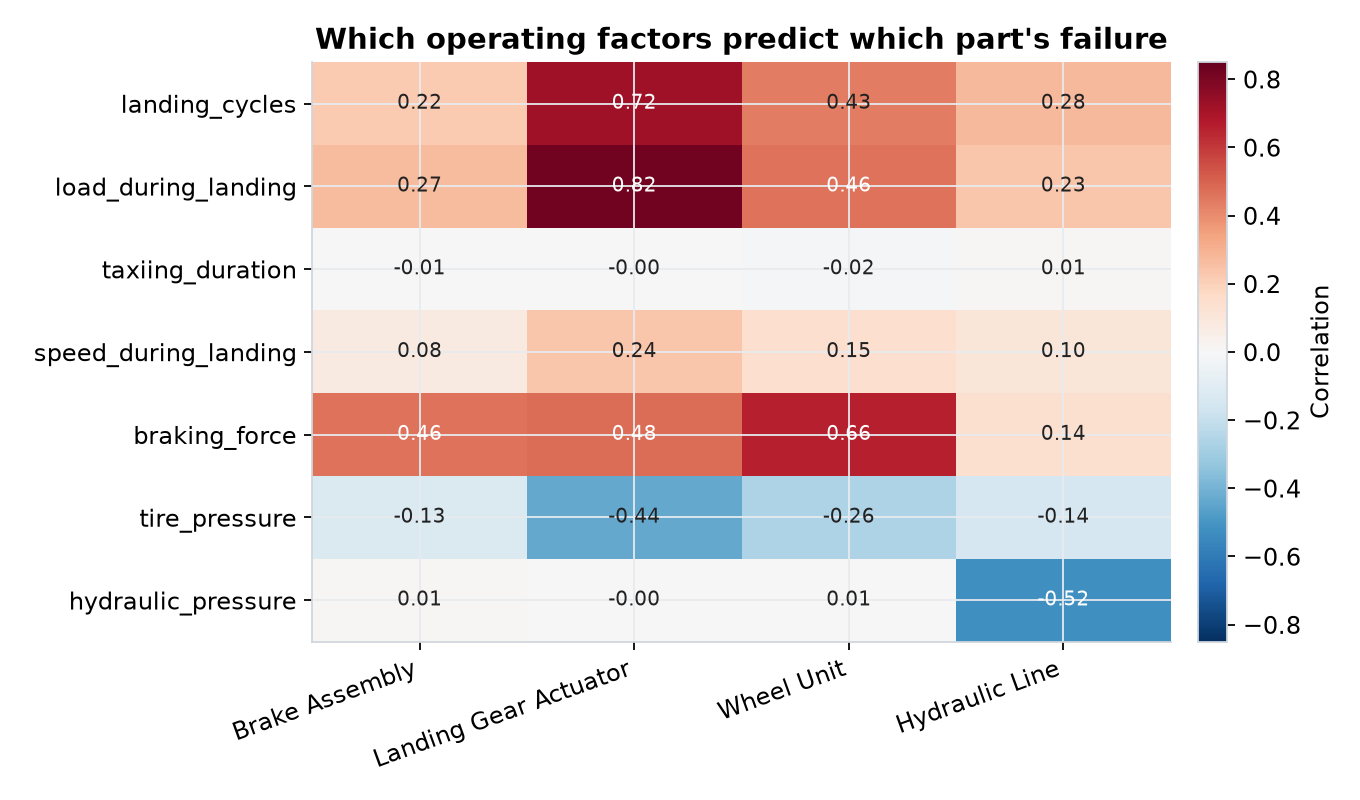
\includegraphics[width=0.85\textwidth]{02_cumulative_wear.png}
\caption[Correlation of landing conditions with part failures]{Correlation between each landing condition and each part's failure flag.}
\label{fig:heat}
\end{figure}

\begin{table}[htbp]
\centering\small
\caption[Correlation of landing conditions with part flags]{Correlation of each landing condition with each part's flag}
\label{tab:corr}
\begin{tabular}{@{}lrrrr@{}}
\toprule
\textbf{Condition} & \textbf{Brake Assy.} & \textbf{Actuator} & \textbf{Wheel Unit} & \textbf{Hydr.\ Line}\\
\midrule
Landing cycles & 0.22 & 0.72 & 0.43 & 0.28\\
Load during landing & 0.27 & \textbf{0.82} & 0.46 & 0.23\\
Taxiing duration & $-$0.01 & 0.00 & $-$0.02 & 0.01\\
Speed during landing & 0.08 & 0.24 & 0.15 & 0.10\\
Braking force & \textbf{0.46} & 0.48 & \textbf{0.66} & 0.14\\
Tyre pressure & $-$0.13 & $-$0.44 & $-$0.26 & $-$0.14\\
Hydraulic pressure & 0.01 & 0.00 & 0.01 & \textbf{$-$0.52}\\
\bottomrule
\end{tabular}
\end{table}

Load and braking force are the strongest links for the actuator, wheel unit and brake assembly. For the hydraulic line, the strongest link is hydraulic pressure. For the actuator, landing cycles (0.72) are only a little weaker than load (0.82), so both matter. All brake assembly links are weak, likely because it is flagged 95\% of the time and so varies very little. Taxiing duration has no link to any part.

\section{Baseline forecast}
\label{sec:baseline}
A \gl{baseline}{baseline} is a simple forecast that any model must beat. Here, the baseline always predicts the average number of actuator flags per batch, which is 119.44. Its \gl{mae}{mean absolute error (MAE)}, the average size of the miss, is 5.52 units per batch (Figure~\ref{fig:baseline}). This average included the batch being predicted, which makes the error look slightly smaller than it really is. The fairer version used in Chapter~\ref{ch:model}, which averages only the training batches, has an error of 6.18.

\begin{figure}[htbp]
\centering
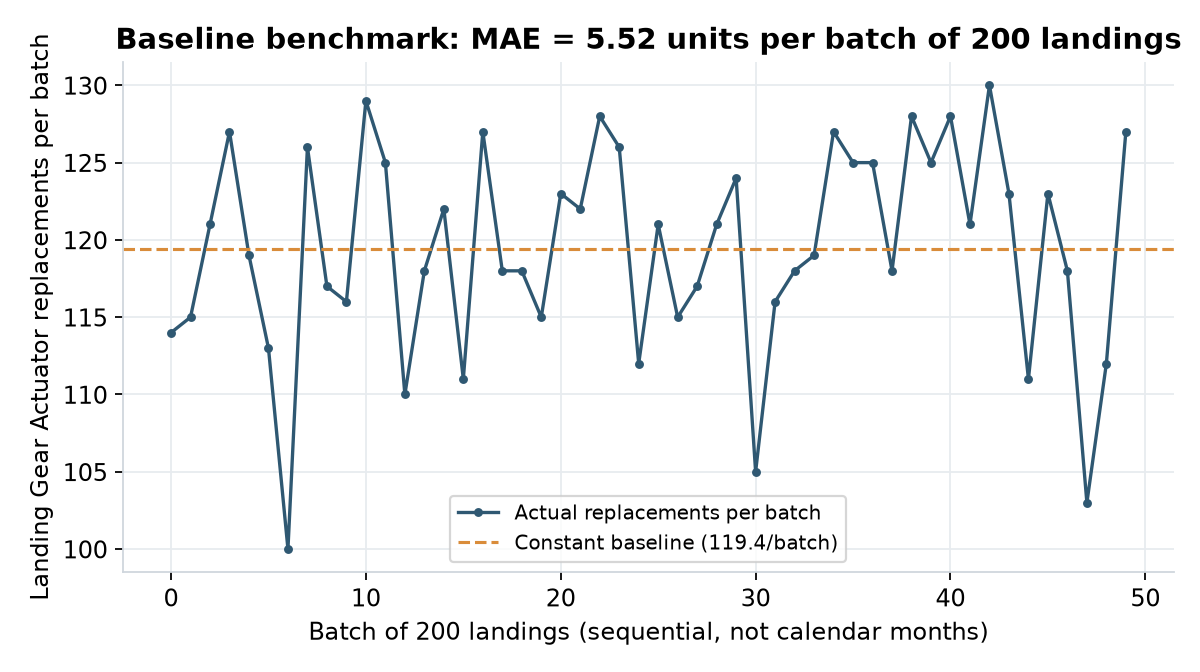
\includegraphics[width=\textwidth]{03_baseline_forecast.png}
\caption[Baseline forecast against actual demand]{Actuator flags per batch of 200 landings compared with the constant-average baseline.}
\label{fig:baseline}
\end{figure}

\section{Value and volatility (ABC/XYZ) classification}
The \gl{abcxyz}{ABC/XYZ classification} ranks parts in two ways. ABC ranks parts by yearly value (number needed per year $\times$ unit cost): A is the highest value, C the lowest. XYZ ranks parts by how steady their demand is, measured by the \gl{cv}{coefficient of variation (CV)}, which is the spread of demand divided by its average. X is the steadiest, Z the most erratic. Standard cut-offs were used: 80\%/95\% of cumulative value for A/B/C, and CV of 0.15/0.30 for X/Y/Z.

Unit costs are assumptions based on public price ranges, converted at \INR 96 per US dollar. Yearly quantities assume 2,000 landings per year. The values are therefore priority scores, not real spending forecasts.

\begin{table}[htbp]
\centering\small
\caption[ABC/XYZ classification of the four parts]{ABC/XYZ classification of the four parts}
\label{tab:abc}
\begin{tabular}{@{}lrrrrc@{}}
\toprule
\textbf{Part} & \textbf{Flag rate} & \textbf{Unit cost (\INR)} & \textbf{Value (\INR cr/yr)} & \textbf{CV} & \textbf{Class}\\
\midrule
Landing Gear Actuator & 59.7\% & 43,20,000 & 516.0 & 0.06 & A/X\\
Brake Assembly & 95.3\% & 17,28,000 & 329.3 & 0.01 & B/X\\
Wheel Unit & 81.7\% & 5,76,000 & 94.1 & 0.03 & C/X\\
Hydraulic Line & 24.5\% & 2,40,000 & 11.8 & 0.12 & C/X\\
\bottomrule
\end{tabular}
\end{table}

\begin{figure}[htbp]
\centering
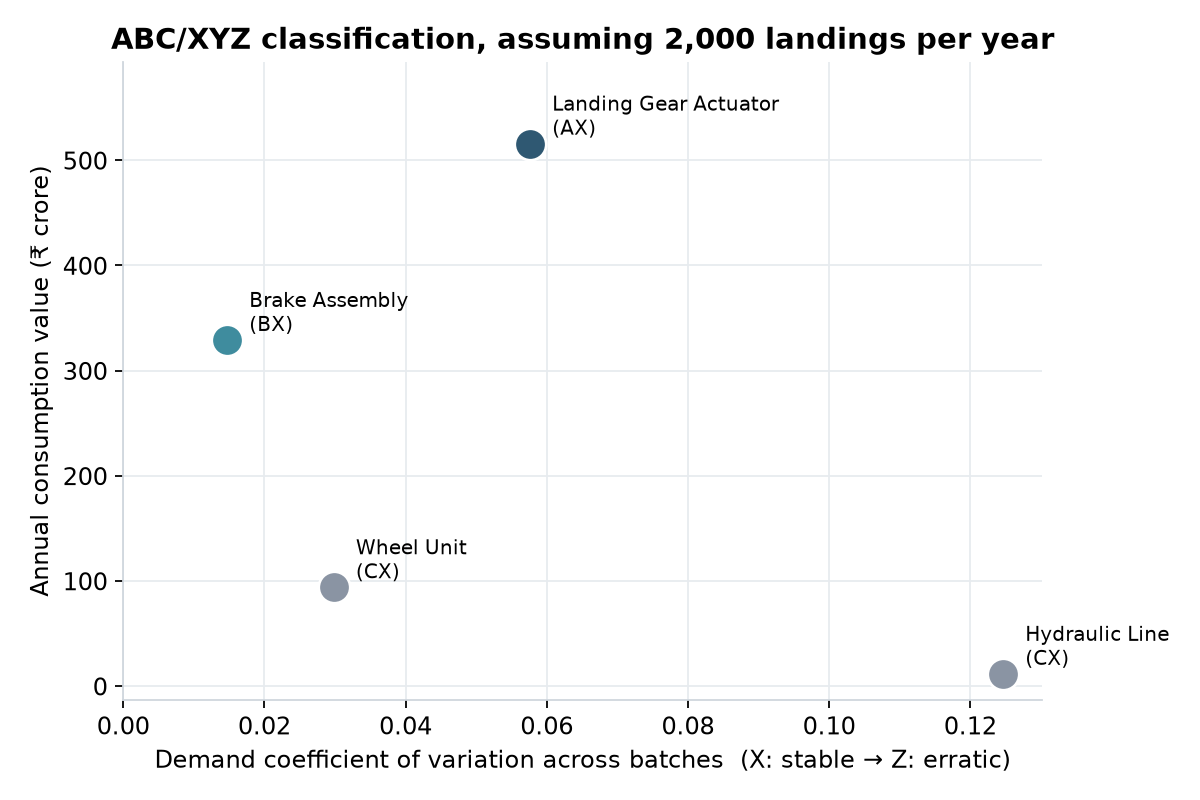
\includegraphics[width=0.85\textwidth]{04_abc_xyz_matrix.png}
\caption[ABC/XYZ classification matrix]{ABC/XYZ matrix. The Landing Gear Actuator is the only Class A/X part.}
\label{fig:abc}
\end{figure}

The Landing Gear Actuator is the only Class A/X part (Table~\ref{tab:abc}, Figure~\ref{fig:abc}): it has the highest value and steady demand. It was therefore chosen as the part to forecast. It was picked because of its value, not because it fails most often; the brake assembly is flagged more often (95.3\%). The original project outline had assumed the brake assembly would be the main part. The classification changed that choice.

\section{Companion parts (Apriori)}
The Apriori algorithm~\cite{agrawal1994} was used to find parts that are flagged together on the same landing. Three measures describe each rule ``when part X is flagged, part Y is also flagged'':
\begin{itemize}
\item \gl{support}{\textbf{support}}: the share of all landings where both parts are flagged;
\item \textbf{confidence}: of the landings where X is flagged, the share where Y is also flagged;
\item \textbf{lift}: how many times more often Y appears with X than it would by chance (above 1 means a real link).
\end{itemize}
With minimum support 0.15 and minimum lift 1.05, three useful rules were found (Table~\ref{tab:apriori}, Figure~\ref{fig:apriori}).

\begin{table}[htbp]
\centering\small
\caption[Companion-part rules]{Companion-part rules found by Apriori}
\label{tab:apriori}
\begin{tabular}{@{}lrrr@{}}
\toprule
\textbf{Rule} & \textbf{Support} & \textbf{Confidence} & \textbf{Lift}\\
\midrule
Hydraulic Line $\rightarrow$ Landing Gear Actuator & 0.18 & 0.72 & 1.20\\
Landing Gear Actuator $\rightarrow$ Wheel Unit & 0.57 & 0.95 & 1.17\\
Hydraulic Line $\rightarrow$ Wheel Unit & 0.21 & 0.87 & 1.07\\
\bottomrule
\end{tabular}
\end{table}

\begin{figure}[htbp]
\centering
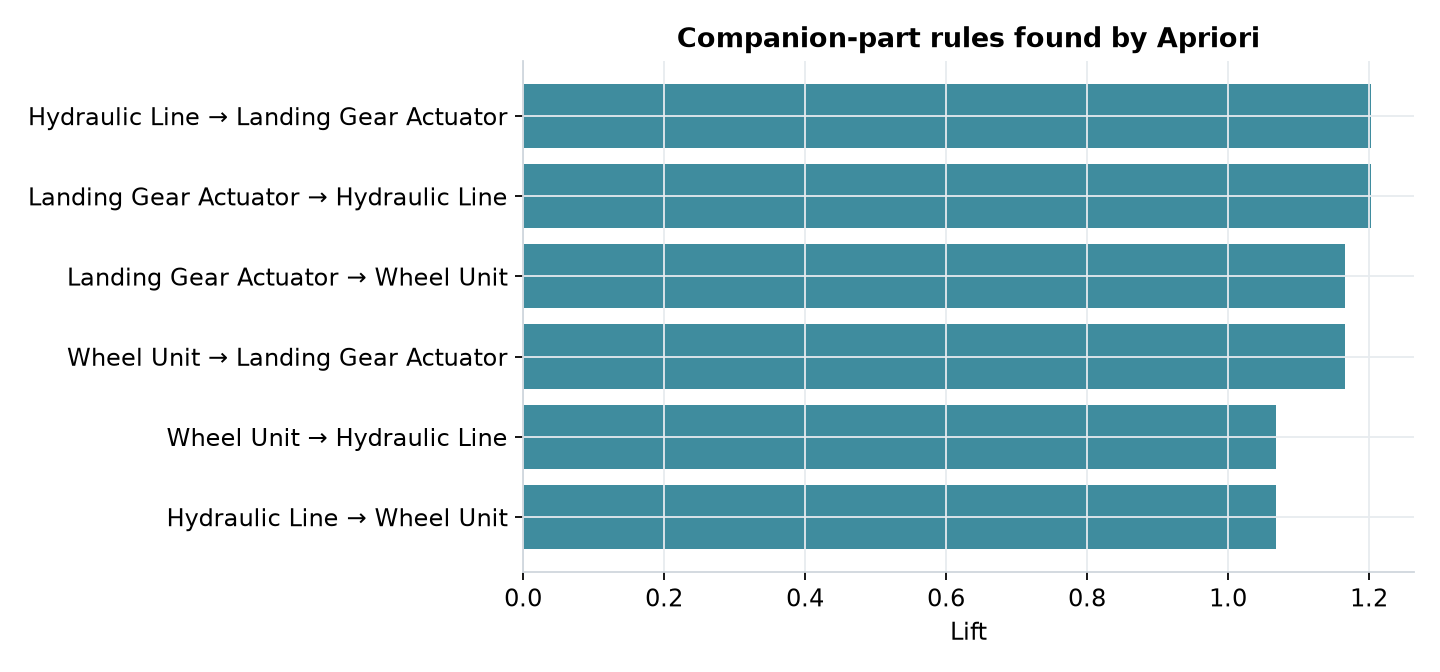
\includegraphics[width=0.85\textwidth]{05_apriori_rules.png}
\caption[Companion-part rules found by Apriori]{Companion-part rules found by Apriori, ranked by lift.}
\label{fig:apriori}
\end{figure}

The most useful rule for a supplier is the second one: when the actuator is flagged, the wheel unit is also flagged 95\% of the time. These links partly come from how the simulator's rules were written (Table~\ref{tab:rules}): landing cycles appears in every rule, and load and braking force are themselves linked (correlation 0.58). On real data, the rules may be weaker or stronger.

\section{Cost of a stockout versus holding stock}
\label{sec:aog}
Table~\ref{tab:aog} shows the cost of one AOG event under three assumed scenarios, each lasting 18 hours.

\begin{table}[htbp]
\centering\small
\caption[AOG cost scenarios]{Assumed AOG cost scenarios (18-hour event, \INR 96 = US\$1)}
\label{tab:aog}
\begin{tabular}{@{}lrr@{}}
\toprule
\textbf{Scenario} & \textbf{AOG cost per hour (\INR)} & \textbf{Cost of one event (\INR)}\\
\midrule
Low (narrow-body, domestic) & 9,60,000 & 1,72,80,000\\
Mid (narrow-body, typical) & 43,20,000 & 7,77,60,000\\
High (wide-body, peak) & 1,44,00,000 & 25,92,00,000\\
\bottomrule
\end{tabular}
\end{table}

The \gl{holding}{holding cost} is assumed to be 25\% of the part's price per year. For one actuator (\INR 43,20,000), this is \INR 10,80,000 per year. Even the Low scenario costs about 16 times that amount for a single event. This is why the stock rule in Chapter~\ref{ch:reorder} aims to avoid stockouts with very high probability.

\begin{figure}[htbp]
\centering
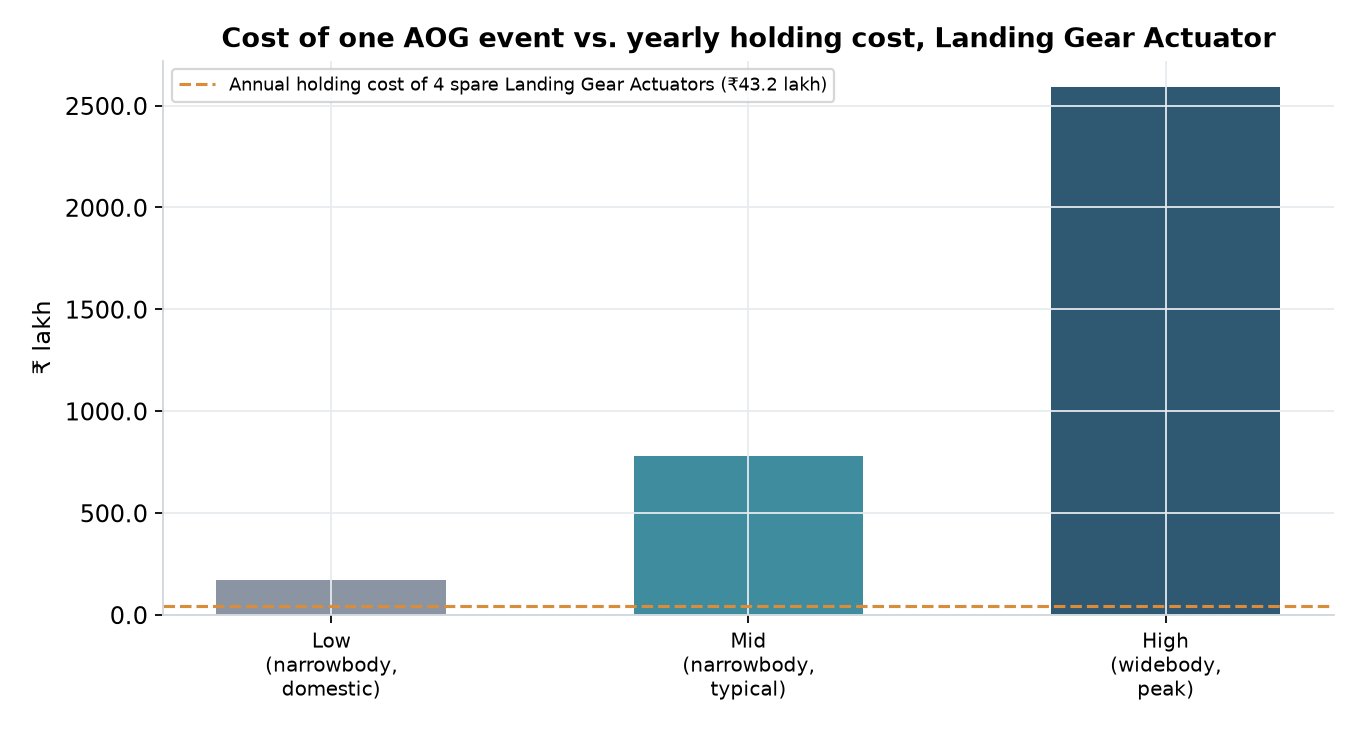
\includegraphics[width=0.85\textwidth]{06_business_case.png}
\caption[AOG event cost against yearly holding cost]{Cost of one AOG event in each scenario compared with the yearly holding cost used in the midterm example.}
\label{fig:aog}
\end{figure}

% ---------------------------------------------------------------------
\chapter{Forecasting Model: Training and Tuning}
\label{ch:model}
% ---------------------------------------------------------------------

\section{Fair testing}
A model must be tested on data it has never seen, otherwise its error looks smaller than it really is. This project uses \gl{cv5}{cross-validation over batches}:
\begin{enumerate}
\item The 50 batches are split at random into 5 groups (``folds'') of 10 batches.
\item The model is trained on the landings in 4 folds (40 batches) and tested on the 5th fold (10 batches) it has never seen.
\item This is repeated 5 times, so every batch is tested exactly once by a model that did not see it.
\end{enumerate}
Whole batches are kept together, so no landing from a test batch is ever used in training.

\section{Tuning}
\gl{tuning}{Hyperparameter tuning} means trying different model settings and keeping the best one. To keep the test fair, tuning was done \emph{only} inside the training batches of each fold. The training batches were split again into 4 inner folds; each setting was trained on 3 and scored on the 4th, using \gl{logloss}{log loss} (a score that punishes confident wrong predictions). The setting with the lowest average log loss was then trained on all training batches and used on the test fold. The settings tried are in Table~\ref{tab:grid}. The grids were kept small and standard; they were not adjusted after seeing the results.

\begin{table}[htbp]
\centering\small
\caption[Settings tried during tuning]{Settings tried during tuning}
\label{tab:grid}
\begin{tabularx}{\textwidth}{@{}lL@{}}
\toprule
\textbf{Model} & \textbf{Settings tried}\\
\midrule
LightGBM (12 combinations) & number of leaves \{7, 15, 31\}; learning rate \{0.03, 0.1\}; number of trees \{100, 300\}; minimum samples per leaf 20\\
Random Forest (6 combinations) & 300 trees; minimum samples per leaf \{1, 5, 20\}; features tried per split \{square root, 60\%\}\\
\bottomrule
\end{tabularx}
\end{table}

LightGBM chose 7 leaves, learning rate 0.03 and 300 trees in four of the five folds (15 leaves in the other). Random Forest chose minimum leaf size 1 and 60\% of features in all five folds. The full list is in Appendix~\ref{app:settings}.

\section{Results}
\label{sec:p5results}
Table~\ref{tab:p5} and Figure~\ref{fig:mae} compare the forecast error per batch.

\begin{table}[htbp]
\centering\small
\caption[Forecast error per batch]{Forecast error per batch of 200 landings (lower is better)}
\label{tab:p5}
\begin{tabular}{@{}lr@{}}
\toprule
\textbf{Method} & \textbf{MAE (units per batch)}\\
\midrule
Midterm baseline (average of all 50 batches) & 5.52\\
Fair baseline (average of training batches only) & 6.18\\
Random Forest (tuned, tested on unseen batches) & \textbf{0.10}\\
LightGBM (tuned, tested on unseen batches) & \textbf{0.30}\\
\bottomrule
\end{tabular}
\end{table}

\begin{figure}[htbp]
\centering
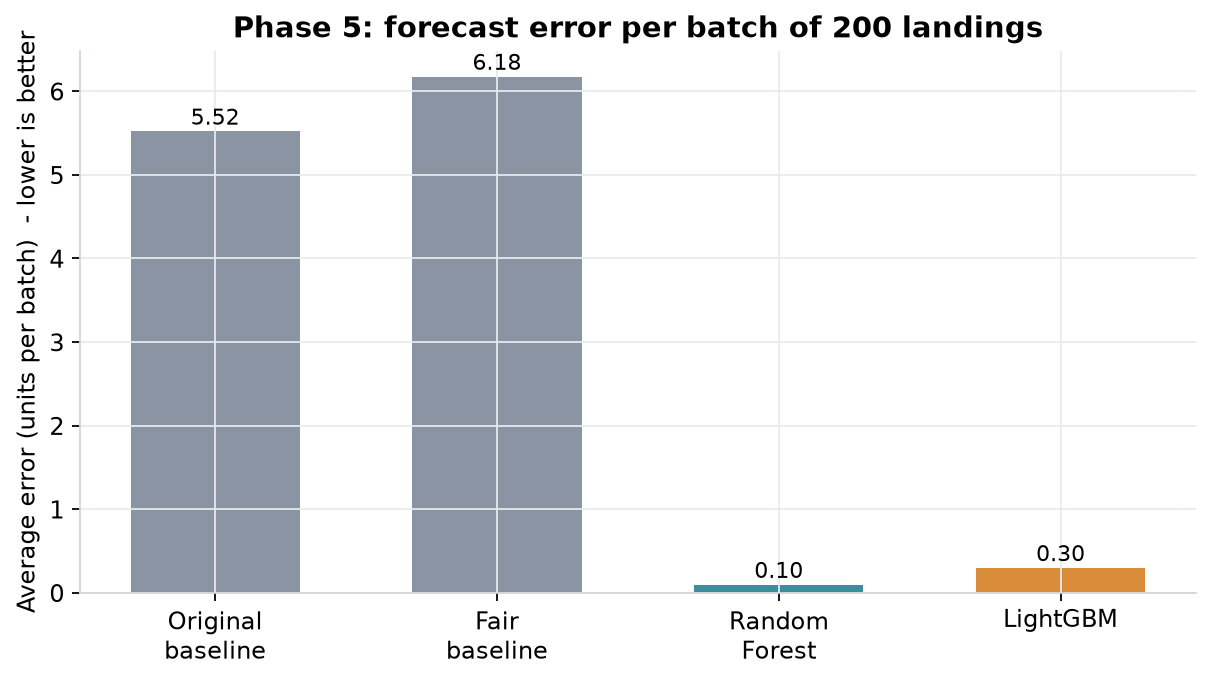
\includegraphics[width=0.8\textwidth]{08_phase5_mae_comparison.png}
\caption[Forecast error by method]{Forecast error (MAE) per batch for each method.}
\label{fig:mae}
\end{figure}

\begin{figure}[htbp]
\centering
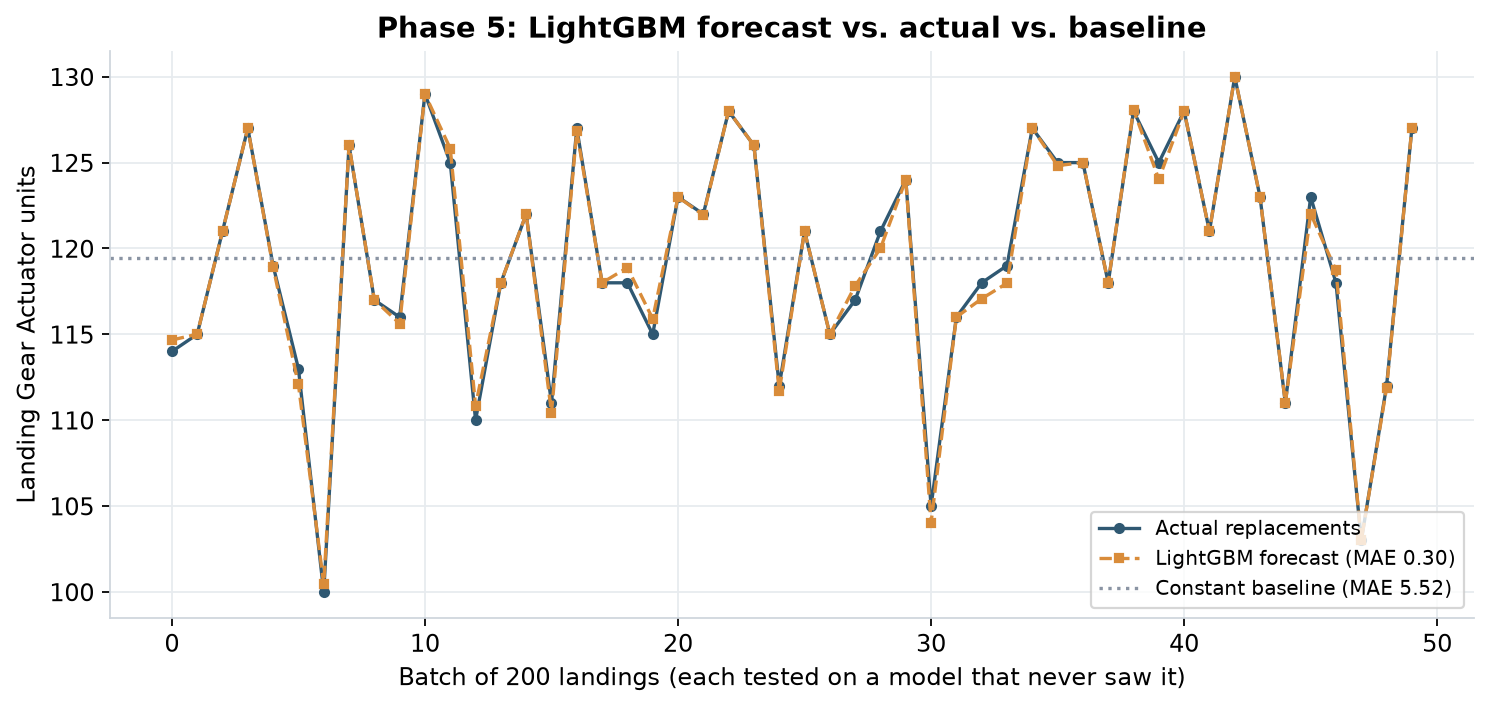
\includegraphics[width=\textwidth]{07_phase5_forecast_vs_actual.png}
\caption[LightGBM forecast against actual demand]{LightGBM forecast compared with actual actuator flags per batch, and the constant baseline. Each batch was forecast by a model that never saw it.}
\label{fig:fva}
\end{figure}

Both models reduce the error from about 6 units to well under 1 unit per batch (Figure~\ref{fig:fva}). At the level of single landings, both models separate failures from non-failures almost perfectly: the \gl{auc}{AUC} (a score from 0.5 for guessing to 1.0 for perfect) is 1.000 for both, and the log loss is 0.0053 for LightGBM and 0.0008 for Random Forest.

\section{Why Random Forest did slightly better}
Random Forest was slightly more accurate than LightGBM (0.10 against 0.30). The likely reason is the sharp cut-off in the simulator's rule (load $>$ 70 or cycles $>$ 401). Random Forest's fully grown trees match a sharp cut-off exactly. LightGBM, with its small learning rate, gives slightly softer chances close to the cut-off. The gap is less than one unit per 200 landings, so it makes no practical difference. LightGBM is kept as the main model because it was chosen in advance for the reasons in Table~\ref{tab:models}, and because on real, noisier data gradient boosting usually performs well~\cite{olmo2026}. This choice should be checked again on real data.

\section{What the model relies on}
\gl{fi}{Feature importance} shows how much each input helped the model. For LightGBM (Figure~\ref{fig:fi}), load during landing accounts for 99.1\% of the total gain and landing cycles for 0.7\%. Every other condition is close to zero, and runway condition is 0.0\%.

\begin{figure}[htbp]
\centering
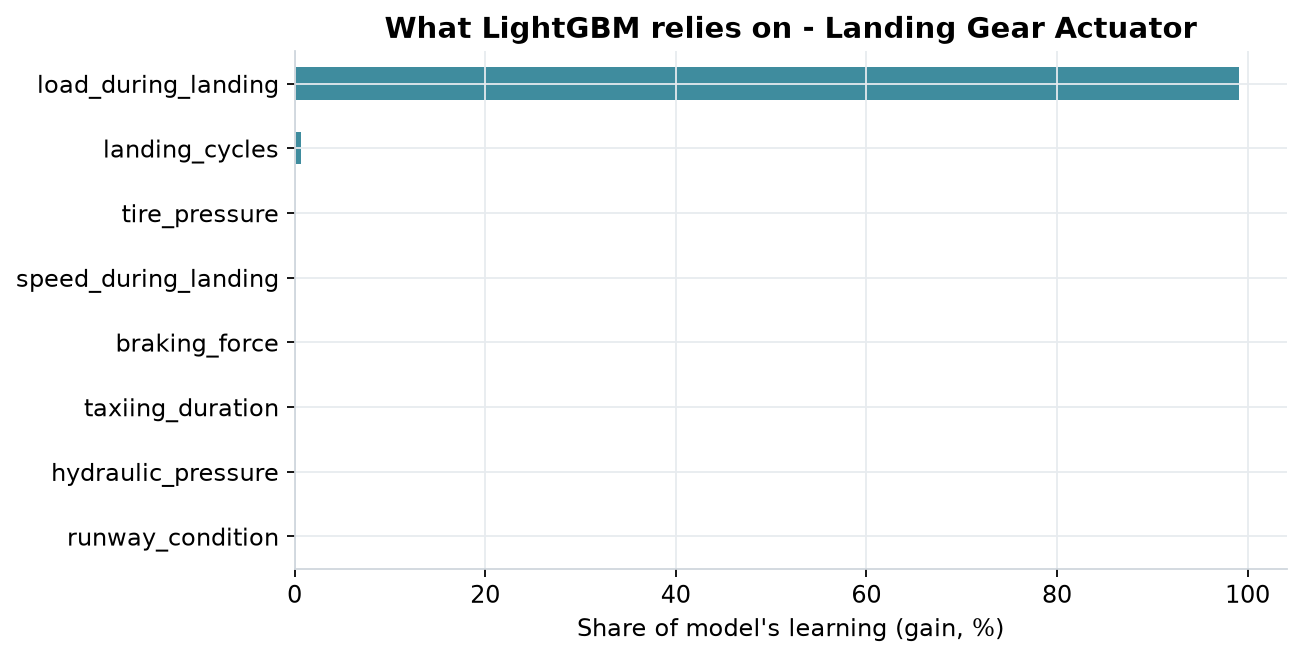
\includegraphics[width=0.8\textwidth]{09_phase5_feature_importance.png}
\caption[LightGBM feature importance]{LightGBM feature importance (share of total gain).}
\label{fig:fi}
\end{figure}

This matches the rule in Table~\ref{tab:rules}: the model found the two conditions the simulator uses and ignored the rest. Load dominates because the two limits overlap: of the 1,982 landings with more than 401 cycles, 1,966 also have load above 70. Only 16 of the 5,972 actuator failures are explained by cycles alone.

\section{Honest reading of these results}
Errors this small are only possible because the flags follow an exact rule with no randomness (Section~\ref{sec:rules}). The best possible error on this data is zero. The results show that the pipeline works correctly and that the fair-testing setup does not leak information. They do \emph{not} show how accurate the model would be on real aircraft.

% ---------------------------------------------------------------------
\chapter{Reorder Engine and Cost Validation}
\label{ch:reorder}
% ---------------------------------------------------------------------

\section{The stock rule}
Before each batch starts, the shelf is filled up to a target level:
\[
\text{target stock} = \text{forecast} + z \times \text{typical forecast error}.
\]
The second part is the \gl{buffer}{safety buffer}. The ``typical forecast error'' is the spread (standard deviation) of each method's past errors, measured only on the \emph{other} folds, never on the batch being planned.

The factor $z$ comes from the \gl{newsvendor}{newsvendor rule}~\cite{silver2017}. It compares two costs:
\begin{itemize}
\item cost of being one unit short = one AOG event (Table~\ref{tab:aog});
\item cost of one extra unit on the shelf for one batch = \INR 43,20,000 $\times$ 25\% $\times$ 0.1 year = \INR 1,08,000.
\end{itemize}
The target chance of \emph{not} running out, the \gl{service}{service level}, is:
\[
\text{service level} = \frac{\text{cost of being short}}{\text{cost of being short} + \text{cost of one extra unit}}.
\]
This gives service levels of 99.38\%, 99.86\% and 99.96\% for the Low, Mid and High scenarios, so $z$ = 2.50, 2.99 and 3.34. Because an AOG event costs so much more than holding a part, the rule aims to have stock almost all the time.

\section{Replaying the 50 batches}
The 50 batches were replayed for three methods: the fair baseline, LightGBM and Random Forest. For each batch, the target stock was compared with the actual demand. Units short were counted as AOG events, and spare units were charged at the holding cost. Results are in Table~\ref{tab:p6} and Figure~\ref{fig:cost}.

\begin{table}[htbp]
\centering\small
\caption[Results of replaying the 50 batches]{Replay of the 50 batches: safety buffer, shortages and yearly cost}
\label{tab:p6}
\begin{tabular}{@{}llrrr@{}}
\toprule
\textbf{Scenario} & \textbf{Method} & \textbf{Avg.\ safety buffer} & \textbf{Batches short} & \textbf{Yearly cost (\INR)}\\
\midrule
Low & Baseline & 19.0 units & 0 of 50 & 2.05 crore\\
    & LightGBM & 1.9 units & 0 of 50 & 20.3 lakh\\
    & Random Forest & 1.0 unit & 0 of 50 & 10.4 lakh\\
\midrule
Mid & Baseline & 22.8 units & 0 of 50 & 2.46 crore\\
    & LightGBM & 2.0 units & 0 of 50 & 21.4 lakh\\
    & Random Forest & 1.0 unit & 0 of 50 & 10.4 lakh\\
\midrule
High & Baseline & 25.4 units & 0 of 50 & 2.74 crore\\
     & LightGBM & 2.1 units & 0 of 50 & 21.8 lakh\\
     & Random Forest & 1.0 unit & 0 of 50 & 10.6 lakh\\
\bottomrule
\end{tabular}
\end{table}

\begin{figure}[htbp]
\centering
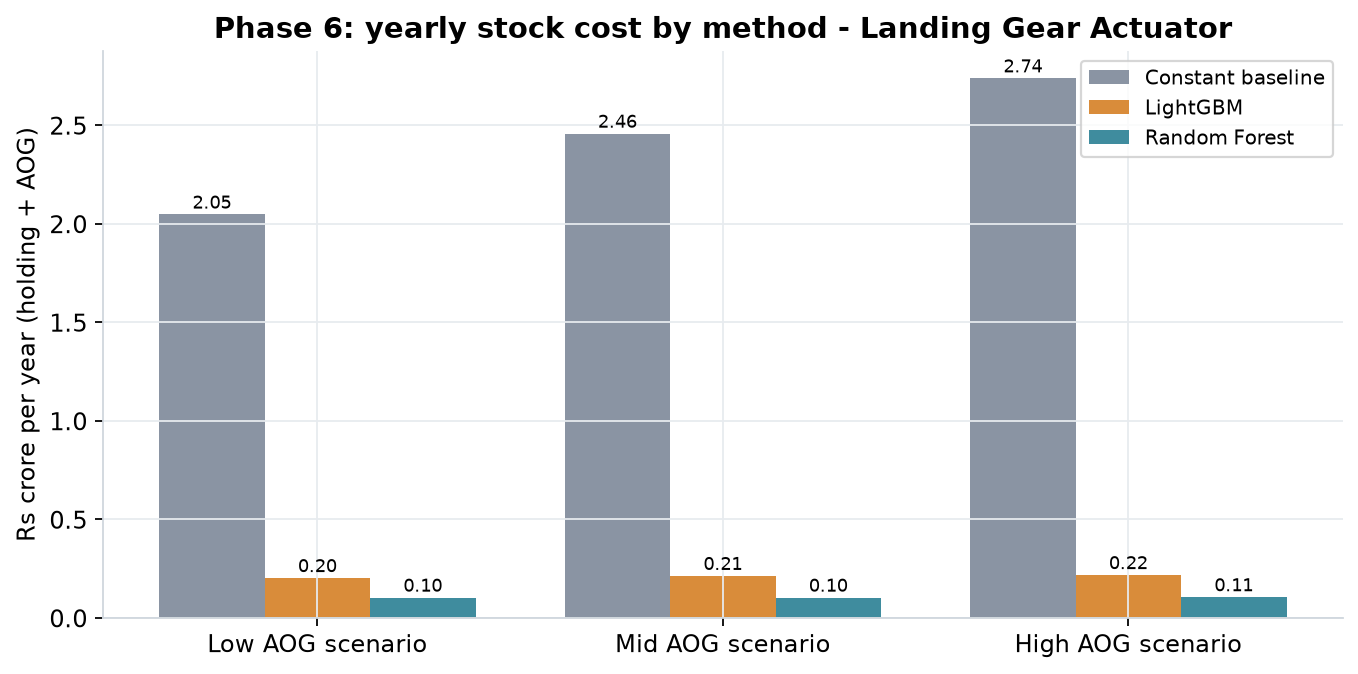
\includegraphics[width=0.85\textwidth]{10_phase6_total_cost.png}
\caption[Yearly cost by method and scenario]{Yearly cost of each method under the three AOG scenarios.}
\label{fig:cost}
\end{figure}

\begin{figure}[htbp]
\centering
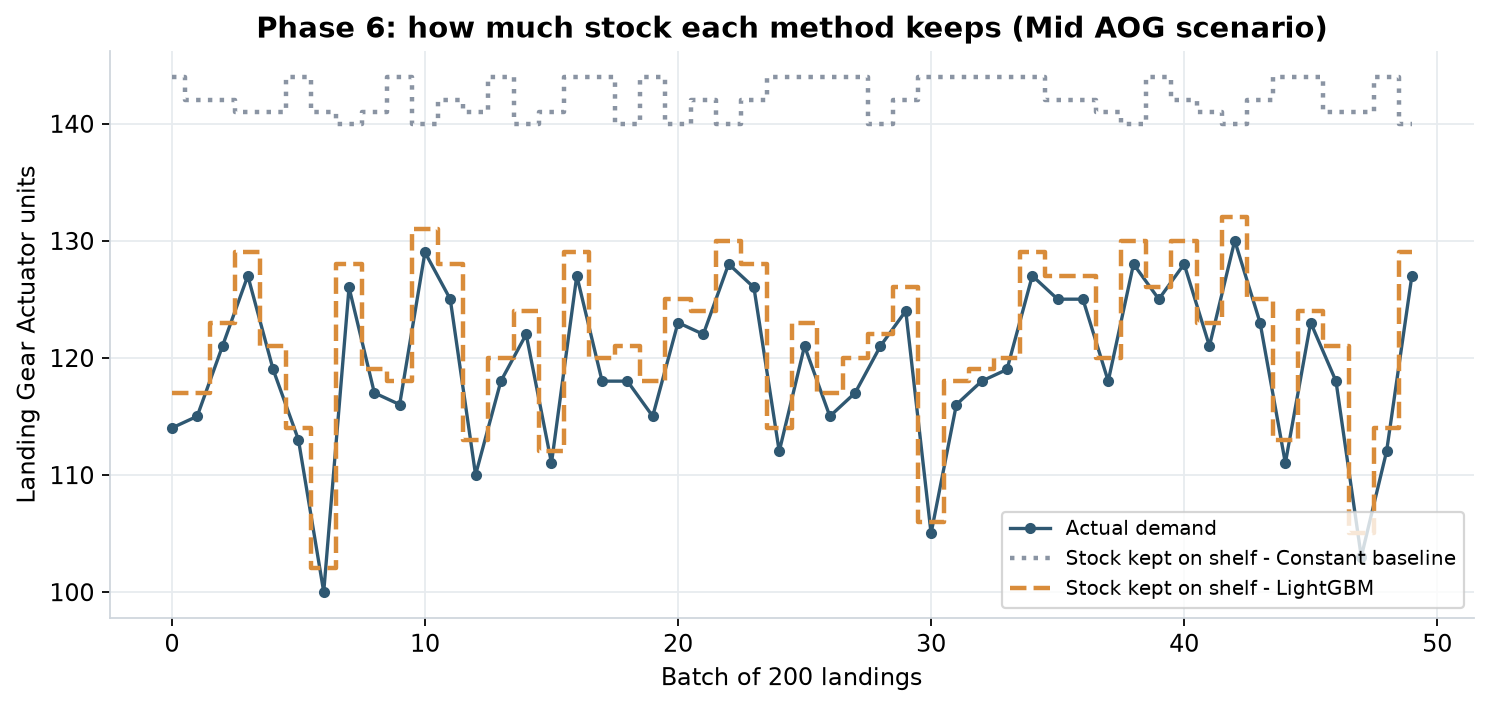
\includegraphics[width=\textwidth]{11_phase6_stock_levels.png}
\caption[Stock kept against actual demand]{Stock kept on the shelf by each method compared with actual demand, Mid scenario.}
\label{fig:stock}
\end{figure}

No method ran short in any of the 50 batches. All of the saving therefore comes from holding fewer spare units for the same protection (Figure~\ref{fig:stock}). With LightGBM, the safety buffer drops from about 23 units to about 2, and the yearly cost drops by about \INR 1.84 crore (Low), \INR 2.24 crore (Mid) and \INR 2.52 crore (High).

Fifty batches is too few to test rare stockouts properly. With a target service level of 99.86\%, a stockout would be expected less than once in 50 batches even if the rule works as designed. The ``0 shortages'' result is encouraging but not proof.

\section{Order size (EOQ)}
The \gl{eoq}{economic order quantity (EOQ)} is the number of units per order that balances the cost of placing orders against the cost of holding stock~\cite{harris1913}:
\[
\text{EOQ} = \sqrt{\frac{2 \times \text{yearly demand} \times \text{cost per order}}{\text{holding cost per unit per year}}}.
\]
Yearly demand is about 1,194 actuators for every method, and the holding cost is \INR 10,80,000 per unit per year. The cost of placing one order (paperwork, transport and inspection) is not known, so a range was tested (Table~\ref{tab:eoq}). \INR 50,000 is the main assumption.

\begin{table}[htbp]
\centering\small
\caption[Order size for different order costs]{Order size (EOQ) for different assumed order costs}
\label{tab:eoq}
\begin{tabular}{@{}rrrr@{}}
\toprule
\textbf{Cost per order (\INR)} & \textbf{EOQ (units)} & \textbf{Orders per year} & \textbf{Orders per batch}\\
\midrule
25,000 & 7 & 171 & 17\\
\textbf{50,000} & \textbf{11} & \textbf{109} & \textbf{11}\\
1,00,000 & 15 & 80 & 8\\
2,00,000 & 21 & 57 & 6\\
\bottomrule
\end{tabular}
\end{table}

EOQ is the same whichever forecast is used, because all methods predict about the same yearly total. The forecast's value is in the safety buffer, not in the order size.

\section{Assumptions behind the cost results}
\begin{itemize}
\item 2,000 landings per year, so one batch is 0.1 year.
\item Parts ordered for a batch arrive before that batch starts (\gl{leadtime}{lead time} is covered by planning one batch ahead).
\item Each unit short is one separate 18-hour AOG event.
\item The forecast uses each landing's conditions. In real use, these would come from flight plans and known cycle counts.
\item Demand is about 119 actuators per 200 landings, because the simulated flag rate is 60\%. This is far higher than for real aircraft, and does not fit well with the ``4 spare units'' holding example used in the midterm report (Figure~\ref{fig:aog}). This is a feature of the simulated data.
\end{itemize}

% ---------------------------------------------------------------------
\chapter{Supplier Dashboard}
\label{ch:dash}
% ---------------------------------------------------------------------

The results are shown in a dashboard built as a single HTML file. It needs no internet connection and no installation; it opens in any web browser. It is created by a script that reads the outputs of Chapters~\ref{ch:model} and~\ref{ch:reorder}, and checks that its yearly costs match those in Table~\ref{tab:p6} before writing the file.

The dashboard has two parts.

\textbf{1. Supplier view} (Figure~\ref{fig:dash}). This part shows only what a supplier needs, using the LightGBM forecast. There is no choice of model, because a supplier does not need one. The user picks a planning batch, an AOG cost scenario and an order cost. Six panels then show:
\begin{itemize}
\item \textbf{Forecast demand}: actuators expected in the batch;
\item \textbf{Stock to keep}: forecast plus safety buffer;
\item \textbf{Safety buffer}: extra units kept in case the forecast is low;
\item \textbf{Order plan}: units per order (EOQ) and orders per batch;
\item \textbf{What actually happened}: actual demand and whether stock was enough;
\item \textbf{Ship together}: the part most often needed with the actuator (Wheel Unit, 95\%).
\end{itemize}
Below these are a chart of stock kept against actual demand for all 50 batches, the list of companion-part rules, and a short ``What the words mean'' section.

\textbf{2. For evaluation.} This part is clearly marked as being for the report and viva, not for suppliers. It compares LightGBM, Random Forest and the baseline: forecast error, safety buffer, shortages and yearly cost.

A banner at the top and a list at the bottom state that the data is simulated and list every cost assumption.

\begin{figure}[htbp]
\centering
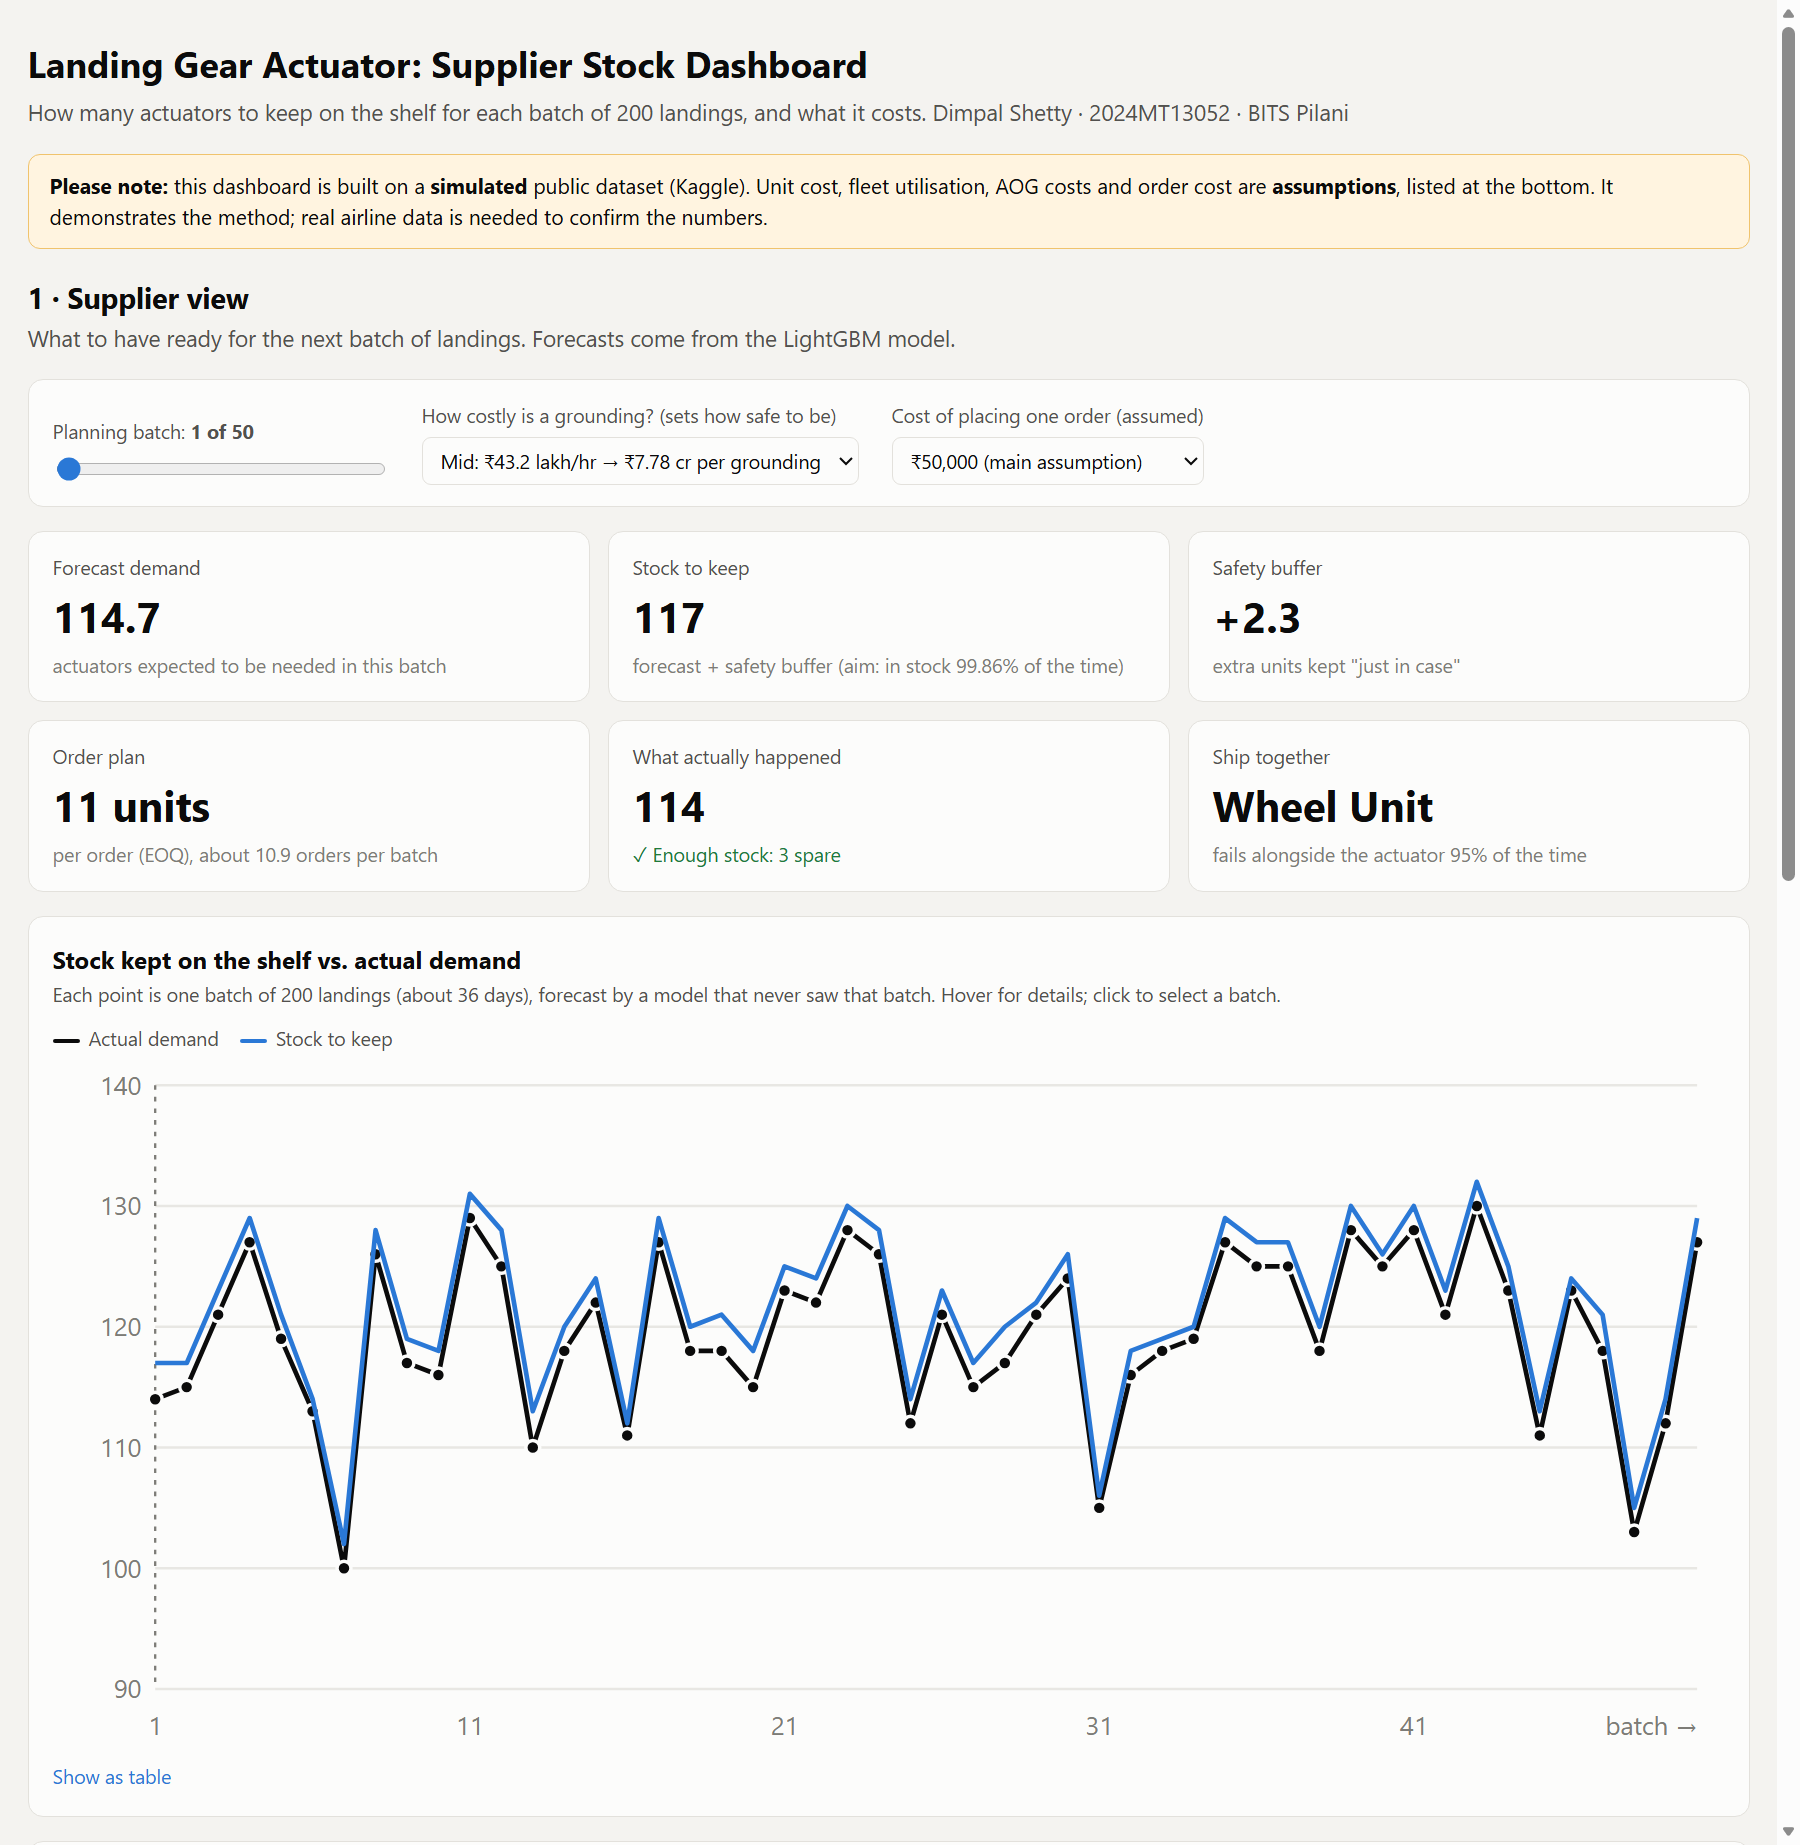
\includegraphics[width=\textwidth]{12_dashboard_supplier_view.png}
\caption[Supplier view of the dashboard]{Supplier view of the dashboard (Mid scenario, batch 1).}
\label{fig:dash}
\end{figure}

% ---------------------------------------------------------------------
\chapter{Limitations}
\label{ch:limits}
% ---------------------------------------------------------------------

\begin{enumerate}
\item \textbf{No real timeline.} The data has no dates or aircraft IDs. Batches of 200 landings stand in for time periods; they are not real months.
\item \textbf{Flags are not confirmed replacements.} A flag probably means ``a problem was detected'', not ``the part was replaced''. Demand figures are therefore an upper estimate.
\item \textbf{Unrealistic demand level.} The simulated actuator flag rate of 60\% gives about 119 actuators per 200 landings, far more than real aircraft would need.
\item \textbf{Assumed costs and usage.} Unit costs, the 25\% holding rate, the AOG cost per hour, the 18-hour event length, the \INR 96 per US dollar exchange rate, the \INR 50,000 order cost and the 2,000 landings per year are all assumptions or public benchmarks, not Airbus figures.
\item \textbf{Too few periods for rare events.} Fifty batches cannot properly test a stock rule designed to run short less than once in several hundred periods.
\item \textbf{Simplified lead time.} The reorder engine assumes orders arrive before each batch starts. Real lead times for actuators can be long and uncertain.
\item \textbf{Only four parts.} Seal kits and structural bolts, named in the original outline, are not in the data.
\item \textbf{Inputs known in advance.} The forecast uses each landing's conditions. In practice, load and cycles must be estimated ahead of time from flight plans and records.
\end{enumerate}

% ---------------------------------------------------------------------
\chapter{Conclusions and Recommendations}
\label{ch:concl}
% ---------------------------------------------------------------------

\section{Conclusions}
\begin{enumerate}
\item A complete pipeline was built, from raw landing data to a stock and order recommendation, and shown in an offline supplier dashboard.
\item The ABC/XYZ classification chose the Landing Gear Actuator as the only high-value, steady-demand part (Class A/X). This replaced the original assumption that the brake assembly was the key part.
\item In this data, landing load and landing cycles drive actuator failure, and runway condition does not. The data check showed this comes from the simulator's rules.
\item Tuned LightGBM and Random Forest models, tested fairly on unseen batches, cut the forecast error from 6.18 to 0.30 and 0.10 units per batch. Random Forest was slightly better on this data; the difference has no practical effect.
\item A cost-based stock rule turned the better forecast into a much smaller safety buffer (about 2 units instead of 23) with no stockouts in the test. This lowered the estimated yearly cost by about \INR 1.8 to 2.5 crore, depending on the AOG scenario.
\item The most useful companion-part rule is that the wheel unit is flagged with the actuator 95\% of the time, which supports bundled orders.
\item The data was found to be simulated, and this was reported openly. The main contribution is therefore the method, which can be re-run unchanged on real data.
\end{enumerate}

\section{Recommendations}
\begin{enumerate}
\item \textbf{Test on real data.} Run the same pipeline on real airline maintenance records with dates, aircraft IDs and confirmed part replacements. This is the most important next step.
\item \textbf{Use real costs and fleet usage.} Replace the assumed landings per year, unit costs, AOG costs and order cost with real figures.
\item \textbf{Model lead time.} Add real supplier lead times, and their variation, to the reorder engine.
\item \textbf{Test over more periods.} Use a longer history to check how often the stock rule really runs short.
\item \textbf{Re-check the model choice.} Compare LightGBM and Random Forest again on real data, where the sharp simulated cut-offs will not exist.
\item \textbf{Extend to more parts.} Apply the same steps to the other parts and to other aircraft systems.
\end{enumerate}

% =====================================================================
%  APPENDICES
% =====================================================================
\appendix
\chapter{Settings Chosen in Each Fold}
\label{app:settings}

\begin{table}[htbp]
\centering\small
\caption[Settings chosen in each fold]{Settings chosen by tuning in each outer fold}
\label{tab:chosen}
\begin{tabular}{@{}clll@{}}
\toprule
\textbf{Fold} & \textbf{Test batches (0-based)} & \textbf{LightGBM} & \textbf{Random Forest}\\
\midrule
1 & 13 17 19 25 26 30 32 39 45 48 & 15 leaves, lr 0.03, 300 trees & leaf 1, 60\% features\\
2 & 3 4 6 8 12 15 37 41 46 47 & 7 leaves, lr 0.03, 300 trees & leaf 1, 60\% features\\
3 & 0 5 9 16 24 27 31 33 34 44 & 7 leaves, lr 0.03, 300 trees & leaf 1, 60\% features\\
4 & 1 2 11 21 23 29 35 36 40 43 & 7 leaves, lr 0.03, 300 trees & leaf 1, 60\% features\\
5 & 7 10 14 18 20 22 28 38 42 49 & 7 leaves, lr 0.03, 300 trees & leaf 1, 60\% features\\
\bottomrule
\end{tabular}
\end{table}

\chapter{Forecasts for Every Batch}
\label{app:batches}

Table~\ref{tab:batches} lists, for each batch, the actual actuator flags, the forecasts of both models, the fair baseline, and the stock that LightGBM would keep in the Mid scenario (``Stock kept''). Stock kept was never below actual demand.

\begin{singlespace}\small
\begin{longtable}{@{}rrrrrr@{}}
\caption[Forecasts for every batch]{Actual and forecast actuator demand for every batch of 200 landings}\label{tab:batches}\\
\toprule
\textbf{Batch} & \textbf{Actual} & \textbf{LightGBM} & \textbf{Random Forest} & \textbf{Fair baseline} & \textbf{Stock kept}\\
\midrule
\endfirsthead
\toprule
\textbf{Batch} & \textbf{Actual} & \textbf{LightGBM} & \textbf{Random Forest} & \textbf{Fair baseline} & \textbf{Stock kept}\\
\midrule
\endhead
1 & 114 & 114.7 & 114.2 & 120.0 & 117\\
2 & 115 & 115.0 & 115.0 & 118.5 & 117\\
3 & 121 & 121.0 & 121.0 & 118.5 & 123\\
4 & 127 & 127.0 & 126.9 & 120.7 & 129\\
5 & 119 & 118.9 & 118.5 & 120.7 & 121\\
6 & 113 & 112.1 & 113.0 & 120.0 & 114\\
7 & 100 & 100.4 & 100.4 & 120.7 & 102\\
8 & 126 & 126.0 & 125.9 & 118.0 & 128\\
9 & 117 & 117.0 & 117.0 & 120.7 & 119\\
10 & 116 & 115.6 & 116.1 & 120.0 & 118\\
11 & 129 & 129.0 & 128.8 & 118.0 & 131\\
12 & 125 & 125.8 & 125.0 & 118.5 & 128\\
13 & 110 & 110.9 & 110.3 & 120.7 & 113\\
14 & 118 & 118.0 & 118.0 & 120.0 & 120\\
15 & 122 & 122.0 & 122.1 & 118.0 & 124\\
16 & 111 & 110.4 & 110.9 & 120.7 & 112\\
17 & 127 & 126.8 & 127.0 & 120.0 & 129\\
18 & 118 & 118.0 & 118.1 & 120.0 & 120\\
19 & 118 & 118.9 & 118.0 & 118.0 & 121\\
20 & 115 & 115.9 & 114.4 & 120.0 & 118\\
21 & 123 & 123.0 & 123.0 & 118.0 & 125\\
22 & 122 & 121.9 & 122.0 & 118.5 & 124\\
23 & 128 & 128.0 & 128.0 & 118.0 & 130\\
24 & 126 & 126.0 & 126.0 & 118.5 & 128\\
25 & 112 & 111.7 & 112.0 & 120.0 & 114\\
26 & 121 & 121.0 & 121.0 & 120.0 & 123\\
27 & 115 & 115.0 & 115.0 & 120.0 & 117\\
28 & 117 & 117.8 & 117.1 & 120.0 & 120\\
29 & 121 & 120.0 & 120.7 & 118.0 & 122\\
30 & 124 & 124.0 & 124.1 & 118.5 & 126\\
31 & 105 & 104.0 & 105.0 & 120.0 & 106\\
32 & 116 & 116.0 & 116.0 & 120.0 & 118\\
33 & 118 & 117.1 & 117.6 & 120.0 & 119\\
34 & 119 & 118.0 & 119.0 & 120.0 & 120\\
35 & 127 & 127.0 & 127.4 & 120.0 & 129\\
36 & 125 & 124.8 & 124.9 & 118.5 & 127\\
37 & 125 & 125.0 & 125.0 & 118.5 & 127\\
38 & 118 & 118.0 & 118.0 & 120.7 & 120\\
39 & 128 & 128.1 & 128.2 & 118.0 & 130\\
40 & 125 & 124.0 & 125.0 & 120.0 & 126\\
41 & 128 & 128.0 & 128.0 & 118.5 & 130\\
42 & 121 & 121.0 & 121.0 & 120.7 & 123\\
43 & 130 & 130.0 & 130.0 & 118.0 & 132\\
44 & 123 & 123.0 & 123.0 & 118.5 & 125\\
45 & 111 & 111.0 & 111.0 & 120.0 & 113\\
46 & 123 & 122.0 & 122.9 & 120.0 & 124\\
47 & 118 & 118.7 & 118.0 & 120.7 & 121\\
48 & 103 & 103.0 & 103.0 & 120.7 & 105\\
49 & 112 & 111.9 & 111.9 & 120.0 & 114\\
50 & 127 & 127.0 & 126.9 & 118.0 & 129\\
\bottomrule
\end{longtable}
\end{singlespace}

% =====================================================================
%  REFERENCES  (numbered in the order they are first cited)
% =====================================================================
\begin{singlespace}
\renewcommand{\bibname}{References}
\begin{thebibliography}{99}
\addcontentsline{toc}{chapter}{References}

\bibitem{bacchetti2012} Bacchetti, A. and Saccani, N., ``Spare parts classification and demand forecasting for stock control: Investigating the gap between research and practice'', \emph{Omega}, Vol.~40, No.~6, 2012, pp.~722-737.

\bibitem{lagoda2024} Lagoda, L. and Klumpp, M., ``Efficient warehouse and inventory management: The modified ABC-XYZ analysis as a framework to integrate demand forecasting and inventory control'', in \emph{Dynamics in Logistics (LDIC 2024)}, Lecture Notes in Logistics, Springer, 2024.

\bibitem{nafiurridha2024} Nafiurridha and Choiruddin, A., ``Classifying MRP strategy of aircraft spare parts using supervised machine learning'', \emph{Procedia Computer Science}, Vol.~234, 2024, pp.~470-477.

\bibitem{olmo2026} Olmo, M.~D. and Domingo, R., ``Intermittent demand forecasting of aerospace rotable parts: A framework for unpredictable flight patterns'', \emph{Computers \& Industrial Engineering}, Vol.~214, 2026.

\bibitem{stanton2025} Stanton, I., Munir, K., Ikram, A. and El-Bakry, M., ``Automation of predictive maintenance: An experimental framework for aircraft landing gear'', \emph{Engineering Reports}, 2025.

\bibitem{agrawal1994} Agrawal, R. and Srikant, R., ``Fast algorithms for mining association rules'', \emph{Proceedings of the 20th International Conference on Very Large Data Bases (VLDB)}, 1994, pp.~487-499.

\bibitem{ke2017} Ke, G., Meng, Q., Finley, T., Wang, T., Chen, W., Ma, W., Ye, Q. and Liu, T.-Y., ``LightGBM: A highly efficient gradient boosting decision tree'', \emph{Advances in Neural Information Processing Systems}, Vol.~30, 2017, pp.~3149-3157.

\bibitem{grinsztajn2022} Grinsztajn, L., Oyallon, E. and Varoquaux, G., ``Why do tree-based models still outperform deep learning on tabular data?'', \emph{Advances in Neural Information Processing Systems}, Vol.~35, 2022, pp.~507-520.

\bibitem{breiman2001} Breiman, L., ``Random Forests'', \emph{Machine Learning}, Vol.~45, No.~1, 2001, pp.~5-32.

\bibitem{silver2017} Silver, E.~A., Pyke, D.~F. and Thomas, D.~J., \emph{Inventory and Production Management in Supply Chains}, 4th edition, Boca Raton: CRC Press, 2017.

\bibitem{harris1913} Harris, F.~W., ``How many parts to make at once'', \emph{Factory, The Magazine of Management}, Vol.~10, No.~2, 1913, pp.~135-136, 152.

\bibitem{kaggle} Eskind, J., ``Landing Gear Predictive Maintenance'', Kaggle dataset (version 1, licence CC0: Public Domain), 2024, \url{https://www.kaggle.com/datasets/justineskind/landing-gear-predictive-maintenance}, accessed 10 September 2026.

\bibitem{pedregosa2011} Pedregosa, F. et al., ``Scikit-learn: Machine learning in Python'', \emph{Journal of Machine Learning Research}, Vol.~12, 2011, pp.~2825-2830.

\bibitem{raschka2018} Raschka, S., ``MLxtend: Providing machine learning and data science utilities and extensions to Python's scientific computing stack'', \emph{Journal of Open Source Software}, Vol.~3, No.~24, 2018, p.~638.

\end{thebibliography}
\end{singlespace}

% =====================================================================
%  GLOSSARY  (term, meaning, page where it is explained)
% =====================================================================
\chapter*{Glossary}
\addcontentsline{toc}{chapter}{Glossary}
\begin{singlespace}
\small
\begin{longtable}{@{}p{3.6cm}p{9.2cm}r@{}}
\toprule
\textbf{Term} & \textbf{Meaning} & \textbf{Page}\\
\midrule
\endhead
ABC/XYZ & Ranking of parts by yearly value (A/B/C) and by how steady demand is (X/Y/Z). & \pageref{gl:abcxyz}\\
AOG & Aircraft On Ground: the aircraft cannot fly because a part is missing. & \pageref{gl:aog}\\
AUC & A score of how well a model separates two outcomes; 0.5 is guessing, 1.0 is perfect. & \pageref{gl:auc}\\
Baseline & A simple forecast (here, a constant average) that a model must beat. & \pageref{gl:baseline}\\
Batch & A group of 200 landings used as one planning period, since the data has no dates. & \pageref{gl:batch}\\
Coefficient of variation (CV) & Spread of demand divided by its average; low means steady demand. & \pageref{gl:cv}\\
Confidence / lift / support & Measures of how strongly two parts are flagged together (Apriori). & \pageref{gl:support}\\
Cross-validation & Testing a model several times, each time on a part of the data it did not train on. & \pageref{gl:cv5}\\
EOQ & Economic Order Quantity: order size that balances ordering cost and holding cost. & \pageref{gl:eoq}\\
Feature importance & How much each input helped the model make its predictions. & \pageref{gl:fi}\\
Holding cost & Cost of keeping a part on the shelf (money tied up, storage, insurance). & \pageref{gl:holding}\\
Hyperparameter tuning & Trying different model settings and keeping the best one. & \pageref{gl:tuning}\\
Lead time & Time between placing an order and receiving the part. & \pageref{gl:leadtime}\\
Log loss & A score that punishes confident wrong predictions; lower is better. & \pageref{gl:logloss}\\
MAE & Mean Absolute Error: the average size of a forecast's miss. & \pageref{gl:mae}\\
MRO & Maintenance, Repair and Overhaul. & \pageref{gl:mro}\\
Newsvendor rule & A rule that sets how much stock to keep by comparing the cost of running short with the cost of extra stock. & \pageref{gl:newsvendor}\\
Safety buffer (safety stock) & Extra units kept on top of the forecast in case demand is higher. & \pageref{gl:buffer}\\
Service level & The target chance of not running out of stock in a period. & \pageref{gl:service}\\
Simulated data & Data produced by a computer program following set rules, not recorded from real events. & \pageref{gl:sim}\\
\bottomrule
\end{longtable}
\end{singlespace}

\end{document}
